\documentclass[lettersize,journal]{IEEEtran}
\usepackage{amsmath,amsfonts}
\usepackage{algorithmic}
\usepackage{algorithm}
\usepackage{array}
\usepackage[caption=false,font=normalsize,labelfont=sf,textfont=sf]{subfig}
\usepackage{textcomp}
\usepackage{stfloats}
\usepackage{url}
\usepackage{verbatim}
\usepackage{graphicx}
\usepackage{cite}
\usepackage{booktabs}
\usepackage{multirow}

\usepackage{amssymb}
\usepackage{bm}
\usepackage[margin=1in]{geometry}

% indicator function
\newcommand{\ind}{\mathbb{1}}
\hyphenation{op-tical net-works semi-conduc-tor IEEE-Xplore}
% updated with editorial comments 8/9/2021

\begin{document}

\title{Hyperbola-Band Attention Supervision for Detection in GPR B-Scan Images}

%\author{IEEE Publication Technology,~\IEEEmembership{Staff,~IEEE,}
        % <-this % stops a space
%\thanks{This paper was produced by the IEEE Publication Technology Group. They are in Piscataway, NJ.}% <-this % stops a space

\author{Ming~Li,
        Christopher~Gomez,
        Shusuke~Miyata,
        and~Norifumi~Hotta
\thanks{M. Li and C. Gomez are with the Sabo Laboratory, Faculty of Maritime Sciences, Kobe University, Kobe, Japan (e-mail: 251we07w@stu.kobe-u.ac.jp; christophergomez@bear.kobe-u.ac.jp).}
\thanks{S. Miyata is with the Disaster Prevention Research Institute, Kyoto University, Kyoto, Japan (e-mail: miyata.shusuke.2e@kyoto-u.ac.jp).}
\thanks{N. Hotta is with the Department of Forest Science, Graduate School of Agricultural and Life Sciences, The University of Tokyo, Tokyo, Japan (e-mail: hotta.norifumi@fr.a.u-tokyo.ac.jp).}


}

% The paper headers
% \markboth{Journal of \LaTeX\ Class Files,~Vol.~14, No.~8, August~2021}%
% {Shell \MakeLowercase{\textit{et al.}}: A Sample Article Using IEEEtran.cls for IEEE Journals}

% Remember, if you use this you must call \IEEEpubidadjcol in the second
% column for its text to clear the IEEEpubid mark.

\maketitle

\begin{abstract}
% 准确识别出B-scan中的双曲线对于掩埋物的参数构建，比如深度、直径等，是核心前提。
% 然而，  导致   。
% 在这个文章中，我们提出了一个   模型，which 结合  能力和  能力去应对B-scan中双曲线检测。
% 还使用   能够   。
% 实验在  数据集上进行验证。
% 结果发现 与   方法相比表现更有，甚至在   下达到   。
% 这些结果说明 使用  能够   
%地质雷达（GPR）B扫描图像中的双曲线回波是目标探测与参数反演的关键依据，但小样本条件下现有方法普遍面临几何信息缺失与注意力漂移的问题。传统检测框仅能粗略刻画回波的空间范围，无法编码顶点位置、曲率、带宽等精细几何特征；而现有注意力机制依赖数据驱动学习，在训练样本有限时难以稳定聚焦于真实双曲线结构，容易偏移至背景杂波。为此，本文提出一种双曲线带注意力监督方法，将标注阶段获得的几何参数转化为对检测网络注意力分支的显式监督信号，从而将目标的几何先验直接注入网络学习过程。具体而言，本文设计了一套面向双曲线带目标的标注工具，用顶点坐标、斜率、水平跨度和带厚度等少量可解释参数描述每条双曲线，并同步导出形状参数与派生矩形框；在此基础上，由参数化标注生成的双曲线带掩码被用于约束注意力分布，实现端到端训练下的检测性能提升。在包含318个样本的公开GPR数据集上的实验表明，该方法在训练比例为0.7时将F1分数从0.68提升至0.84，模型稳定性显著增强，并优于多种主流注意力模块，验证了所提方法的有效性。

In ground penetrating radar (GPR) B-scan images, subsurface targets appear as hyperbolic reflections, and their accurate detection is a prerequisite for target localization and parameter inversion. 
Existing deep learning detectors typically adopt axis-aligned bounding boxes as the annotation format, overlooking the strip-like, symmetric, and parametric geometry of hyperbolic echoes. 
Moreover, the purely data-driven nature of existing attention mechanisms makes attention maps prone to drift under few-shot conditions, deviating from true hyperbolic structures and being misled by background clutter, which ultimately undermines detection stability. 
To address these issues, this paper proposes a hyperbola-band attention supervision method. 
We develop the hyperbola-band annotation tool (HBAT), 
a dedicated annotation tool that represents each target as a parametric band defined by its vertex, slope, span, and thickness. From these parameters, HBAT simultaneously rasterizes a band mask and derives the corresponding bounding box, ensuring geometric consistency between the two label types.
Building on these annotations, an attention branch in the network learns to focus on hyperbola regions under the explicit supervision of this mask, and the resulting spatial prior is injected into the detection features, with the whole network trained end to end. 
Experiments on a public GPR dataset show that the proposed method consistently outperforms the baseline across training-data ratios, 
with the largest gain raising the F1-score from 0.68 to 0.84, 
while substantially reducing variance across random seeds. 
The method also surpasses four representative data-driven attention modules, 
demonstrating the effectiveness of explicit geometric supervision for hyperbola detection in GPR B-scans, 
with consistent gains confirmed on an additional GPR dataset..
%Experiments on a public GPR dataset show that the proposed method consistently outperforms the baseline across training-data ratios, raising the F1-score from 0.68 to 0.84 at best with markedly improved training stability, and surpasses representative self-learned attention modules, demonstrating the effectiveness of explicit geometric supervision for hyperbola detection in GPR B-scans.

\end{abstract}

\begin{IEEEkeywords}
Ground penetrating radar (GPR), hyperbola detection, attention supervision, deep learning.
\end{IEEEkeywords}

\section{Introduction}
% 随着城市地下空间精细化管理、交通基础设施服役状态评估与岩土工程勘察的需求不断提升，高效可靠的地下无损探测技术已成为工程领域的重要研究方向。探地雷达（Ground Penetrating Radar, GPR）凭借非侵入、探测效率高、分辨率适中等技术优势，广泛应用于地下管线探测、道路内部病害检测、隧道衬砌质量检测与隐蔽工程勘察等场景。实际探测中，天线沿测线移动并在每个位置发射电磁脉冲、采集地下介质的反射回波；将连续的单道回波数据沿测线方向并排堆叠，便得到二维 B-scan 图像。其横轴对应天线的空间位置，纵轴对应电磁波的双程走时，可等效为地下深度。
% 对于管线、钢筋等紧凑地下目标，当天线位于其正上方时电磁波往返路径最短、对应走时最小，向两侧移动时路径对称增大、走时随之增加，因此其反射回波在 B-scan 中呈现为开口向下的双曲线，顶点即对应目标的正上方投影。也正因如此，双曲线检测成为地下目标定位、埋深估计与参数重建的关键前置步骤。


% 早期双曲线检测主要依赖手工设计特征与解析曲线拟合，例如 Hough 变换投票、预设模板匹配、HOG 特征结合 SVM 分类等。这类方法在理想实验条件下具备明确的可解释性，但工程局限性突出：不仅计算开销大、对参数离散精度敏感，且检测效果强依赖人工预设的先验模板，面对地下介质不均、杂波干扰强的现场实测数据时，性能衰减十分明显。

% 随着深度学习的发展，端到端的目标检测方法被广泛迁移至 B-scan 双曲线识别任务，在检测效率与定位精度上取得了显著提升。但现有研究普遍直接沿用面向自然图像的矩形框作为标注与输出形式，并未针对双曲线的几何特性做适配。矩形框仅能粗略框定回波的空间范围，其内部包含大量非目标背景区域，既无法提供顶点位置、曲率、条带厚度等精细的几何监督信息，也使得模型难以聚焦于双曲线本身的结构特征进行学习，制约了检测精度的进一步提升，也导致模型在数据量有限的场景下稳定性较差。

% 与此同时，注意力机制已成为提升 GPR 双曲线检测性能的常用技术手段通过通道或空间维度的特征重加权实现注意力分配,增强目标相关特征、抑制无关背景噪声。但由于缺乏明确的目标几何先验引导，效果并不稳定。

% 针对上述不足,本文提出一种双曲线带注意力监督方法:在标注端以少量参数直接记录双曲线的几何形状,在学习端将该几何信息转化为注意力分支的监督信号,提升检测性能。本文的主要贡献如下:

% 1.设计了一种面向双曲线带状目标的专用标注工具。该工具以顶点坐标、斜率、跨度、厚度等少量可解释参数定义双曲线条带，支持交互式快速调整，可同步导出形状参数与派生矩形边界框。
% 2.提出了一种基于几何先验的显式注意力监督机制。通过参数化标注生成的双曲线条带掩膜直接约束注意力分布，为检测网络注入明确的目标空间先验，在端到端训练中提升检测性能.


\IEEEPARstart 
{A}s a widely recognized non-destructive inspection technique, Ground Penetrating Radar (GPR) provides high-resolution, near-real-time imaging of internal structures by employing high-frequency electromagnetic waves, allowing researchers and engineers to visualize features embedded within otherwise opaque media~\cite{Benedetto2017An}. 
GPR radargram interpretation thus extends well beyond conventional geological surveys, constituting a key technology underlying a wide range of applications, 
including infrastructure maintenance, archaeological interpretation, military operations~\cite{Bai2023A}, and driftwood monitoring in river systems~\cite{gomez}. 

In GPR B-scan images, hyperbolic reflection patterns are a hallmark of discrete subsurface objects such as pipes, boulders, and driftwood. The shape of these hyperbolas encodes depth and size. Accurately identifying these hyperbolas is therefore essential for reliable target detection and parameter inversion~\cite{Dou2016Real-Time}.

%In GPR B-scan images, discrete subsurface targets such as pipes, boulders, and driftwood exhibit approximately hyperbolic reflection patterns. Their shape encodes depth and size. Reliable identification of hyperbolas is therefore a essential for GPR target detection and parameter inversion ~\cite{Dou2016Real-Time}. 

%{W}{ith} the growing demand for refined management of urban underground space, service condition assessment of transportation infrastructure, and geotechnical engineering investigation, efficient and reliable underground nondestructive testing technologies have become a prominent research direction in the engineering field~\cite{lai2018review}. Ground Penetrating Radar (GPR), favored for its non-intrusive nature, high survey efficiency, and moderate spatial resolution, is widely applied in scenarios such as underground pipeline detection, road internal defect inspection, tunnel lining quality assessment, and concealed engineering investigation~\cite{rasol2022road,travassos2021review}. 
%During field surveys, the antenna moves along a survey line, emitting electromagnetic pulses and collecting reflected echoes from subsurface media at each position. By stacking consecutive single-trace echoes side by side along the survey line, a two-dimensional B-scan image is obtained, where the horizontal axis corresponds to the spatial position of the antenna, and the vertical axis represents the two-way travel time of electromagnetic waves, which can be equivalently converted to subsurface depth.For compact subsurface targets such as pipelines and rebars, the round-trip path of electromagnetic waves is the shortest when the antenna is directly above the target, corresponding to the minimum travel time. As the antenna moves laterally away from the target, the path length increases symmetrically and the travel time rises accordingly. As a result, the reflected echoes of such targets appear as downward-opening hyperbolas in B-scan images, with the apex corresponding to the vertical projection of the target. For this reason, hyperbola detection serves as a critical prerequisite for subsurface target localization, depth estimation, and parameter reconstruction~\cite{tong2020survey}.

%Early hyperbola detection methods mainly relied on hand-crafted features and analytical curve fitting, typical examples including Hough transform voting, predefined template matching, and HOG features combined with SVM classification~\cite{travassos2021review}. While these methods offer clear interpretability under ideal experimental conditions, they suffer from notable practical limitations: they incur high computational costs, are sensitive to the discretization precision of parameters, and their performance heavily depends on manually designed prior templates~\cite{tong2020survey}. When applied to field data with heterogeneous subsurface media and strong clutter interference, their performance degrades significantly.

Early hyperbola detection methods relied on hand-crafted features and analytical curve fitting~\cite{travassos2021review}, but their performance is highly sensitive to manually designed priors and degrades significantly under heterogeneous subsurface conditions~\cite{tong2020survey}. 
Deep learning has since become the dominant paradigm~\cite{besaw2015deep,redmon2016yolo}, yet its effectiveness relies on large-scale, well-annotated training data,  rarely available in practical GPR surveys due to the high cost of data collection and expert annotation. Moreover, standard detectors rely on rectangular bounding boxes that only coarsely delineate the spatial extent of an echo, without encoding fine-grained geometric properties of hyperbolas, such as vertex position, curvature, and band thickness. This structural information loss limits the network's ability to learn target-specific cues, and becomes especially detrimental under few-shot conditions, where limited training samples leave the model with no means to compensate for the missing geometric guidance, resulting in severe overfitting and unstable performance.

To steer the model toward real hyperbola structures and suppress background clutter,attention mechanisms have been introduced to help models focus on target regions~\cite{hu2018senet,woo2018cbam,wang2020eca,hou2021coordinate,Fu2024A,hou2025endtoend}. They reweight features along the channel or spatial dimensions.
These mechanisms are typically implicit and data-driven, and learning where to attend is itself an additional burden on top of the primary detection task~\cite{Hsiao2025ResNet-SE-CBAM}. Under few-shot conditions, the network has too little data to calibrate both the detection backbone and the attention weights~\cite{XIN2024102307}, so attention maps tend to deviate from the actual hyperbolic structures and become diluted by background clutter. 
%有没有小样本下使用先验知识的理论支持或者案例
%With the development of deep learning, end-to-end object detection methods have been widely adapted for B-scan hyperbola recognition~\cite{besaw2015deep,redmon2016yolo,redmon2018yolov3,bochkovskiy2020yolov4}, delivering remarkable improvements in detection efficiency and localization accuracy. 
%However, standard deep learning paradigms inherently rely on a massive amount of well-labeled training data to guarantee accuracy and robustness.In practical GPR surveys, collecting and annotating substantial real-world datasets is often labor-intensive and constrained by specialist availability. Under few-shot scenarios (i.e., extremely limited data), standard models suffer from severe overfitting.
%Moreover, existing studies generally adopt rectangular bounding boxes designed for natural images as the annotation and output format~\cite{redmon2016yolo}, without tailoring the scheme to the geometric properties of hyperbolas. A rectangular box can only roughly delineate the spatial range of an echo, enclosing a large amount of non-target background area. It neither provides fine-grained geometric supervision such as vertex position, curvature, or band thickness, nor enables the model to focus on learning the structural characteristics of hyperbolas themselves, which restricts further improvement of detection accuracy and leads to poor model stability in scenarios with limited data.
%To steer the model toward real hyperbola structures and suppress background clutter, attention mechanisms have widely been integrated into GPR hyperbola detection~\cite{hu2018senet,woo2018cbam,wang2020eca,hou2021coordinate,vaswani2017attention,wang2018nonlocal}. They reweight features along the channel or spatial dimensions to amplify target-relevant features and suppress irrelevant background noise. Nevertheless, most existing attention mechanisms are inherently data-driven and implicit. Under few-shot constraints, the network lacks sufficient data to autonomously calibrate its weights, causing the attention map to either dissolve into background clutter or shift away from the true hyperbolic features. Without explicit guidance from target geometric priors, these implicit attention weights remain inconsistent and unreliable across complex underground scenarios, failing to salvage the performance drop caused by limited data.

To address the aforementioned limitations, this paper proposes a hyperbola-band attention supervision method. 
On the annotation side, the geometric shape of each hyperbola is encoded with a small set of parameters; on the learning side, this geometric information is converted into supervisory signals for an attention branch to boost detection performance. 

The main contributions of this work are summarized as follows:
\begin{enumerate}
\item 
 A hyperbola-band annotation tool (HBAT) is developed for labeling hyperbola-band targets in GPR images. Each target is parameterized by a compact set of interpretable attributes: apex position, curvature (slope), lateral span, and band thickness, supporting interactive adjustment during annotation. The tool exports both shape parameters and derived rectangular bounding boxes simultaneously, eliminating the need for separate manual labeling of the two representations.

\item An explicit attention supervision mechanism based on geometric priors is proposed. 
Hyperbola-band masks generated from parametric annotations directly constrain the attention distribution, 
injecting explicit spatial priors of targets into the detection network and improving detection performance via end-to-end training.
\item Experiments on a public GPR dataset of limited scale (318 samples in total) show that the proposed method improves the F1-score from 0.68 to 0.84 at a training ratio of 0.7, with a notable enhancement in model stability. It also outperforms multiple mainstream attention modules, which validates the effectiveness of the proposed method.
\end{enumerate}

\section{Related work}
\subsection{GPR Hyperbola Detection Methodologies}
\begin{figure*}[]
\centering
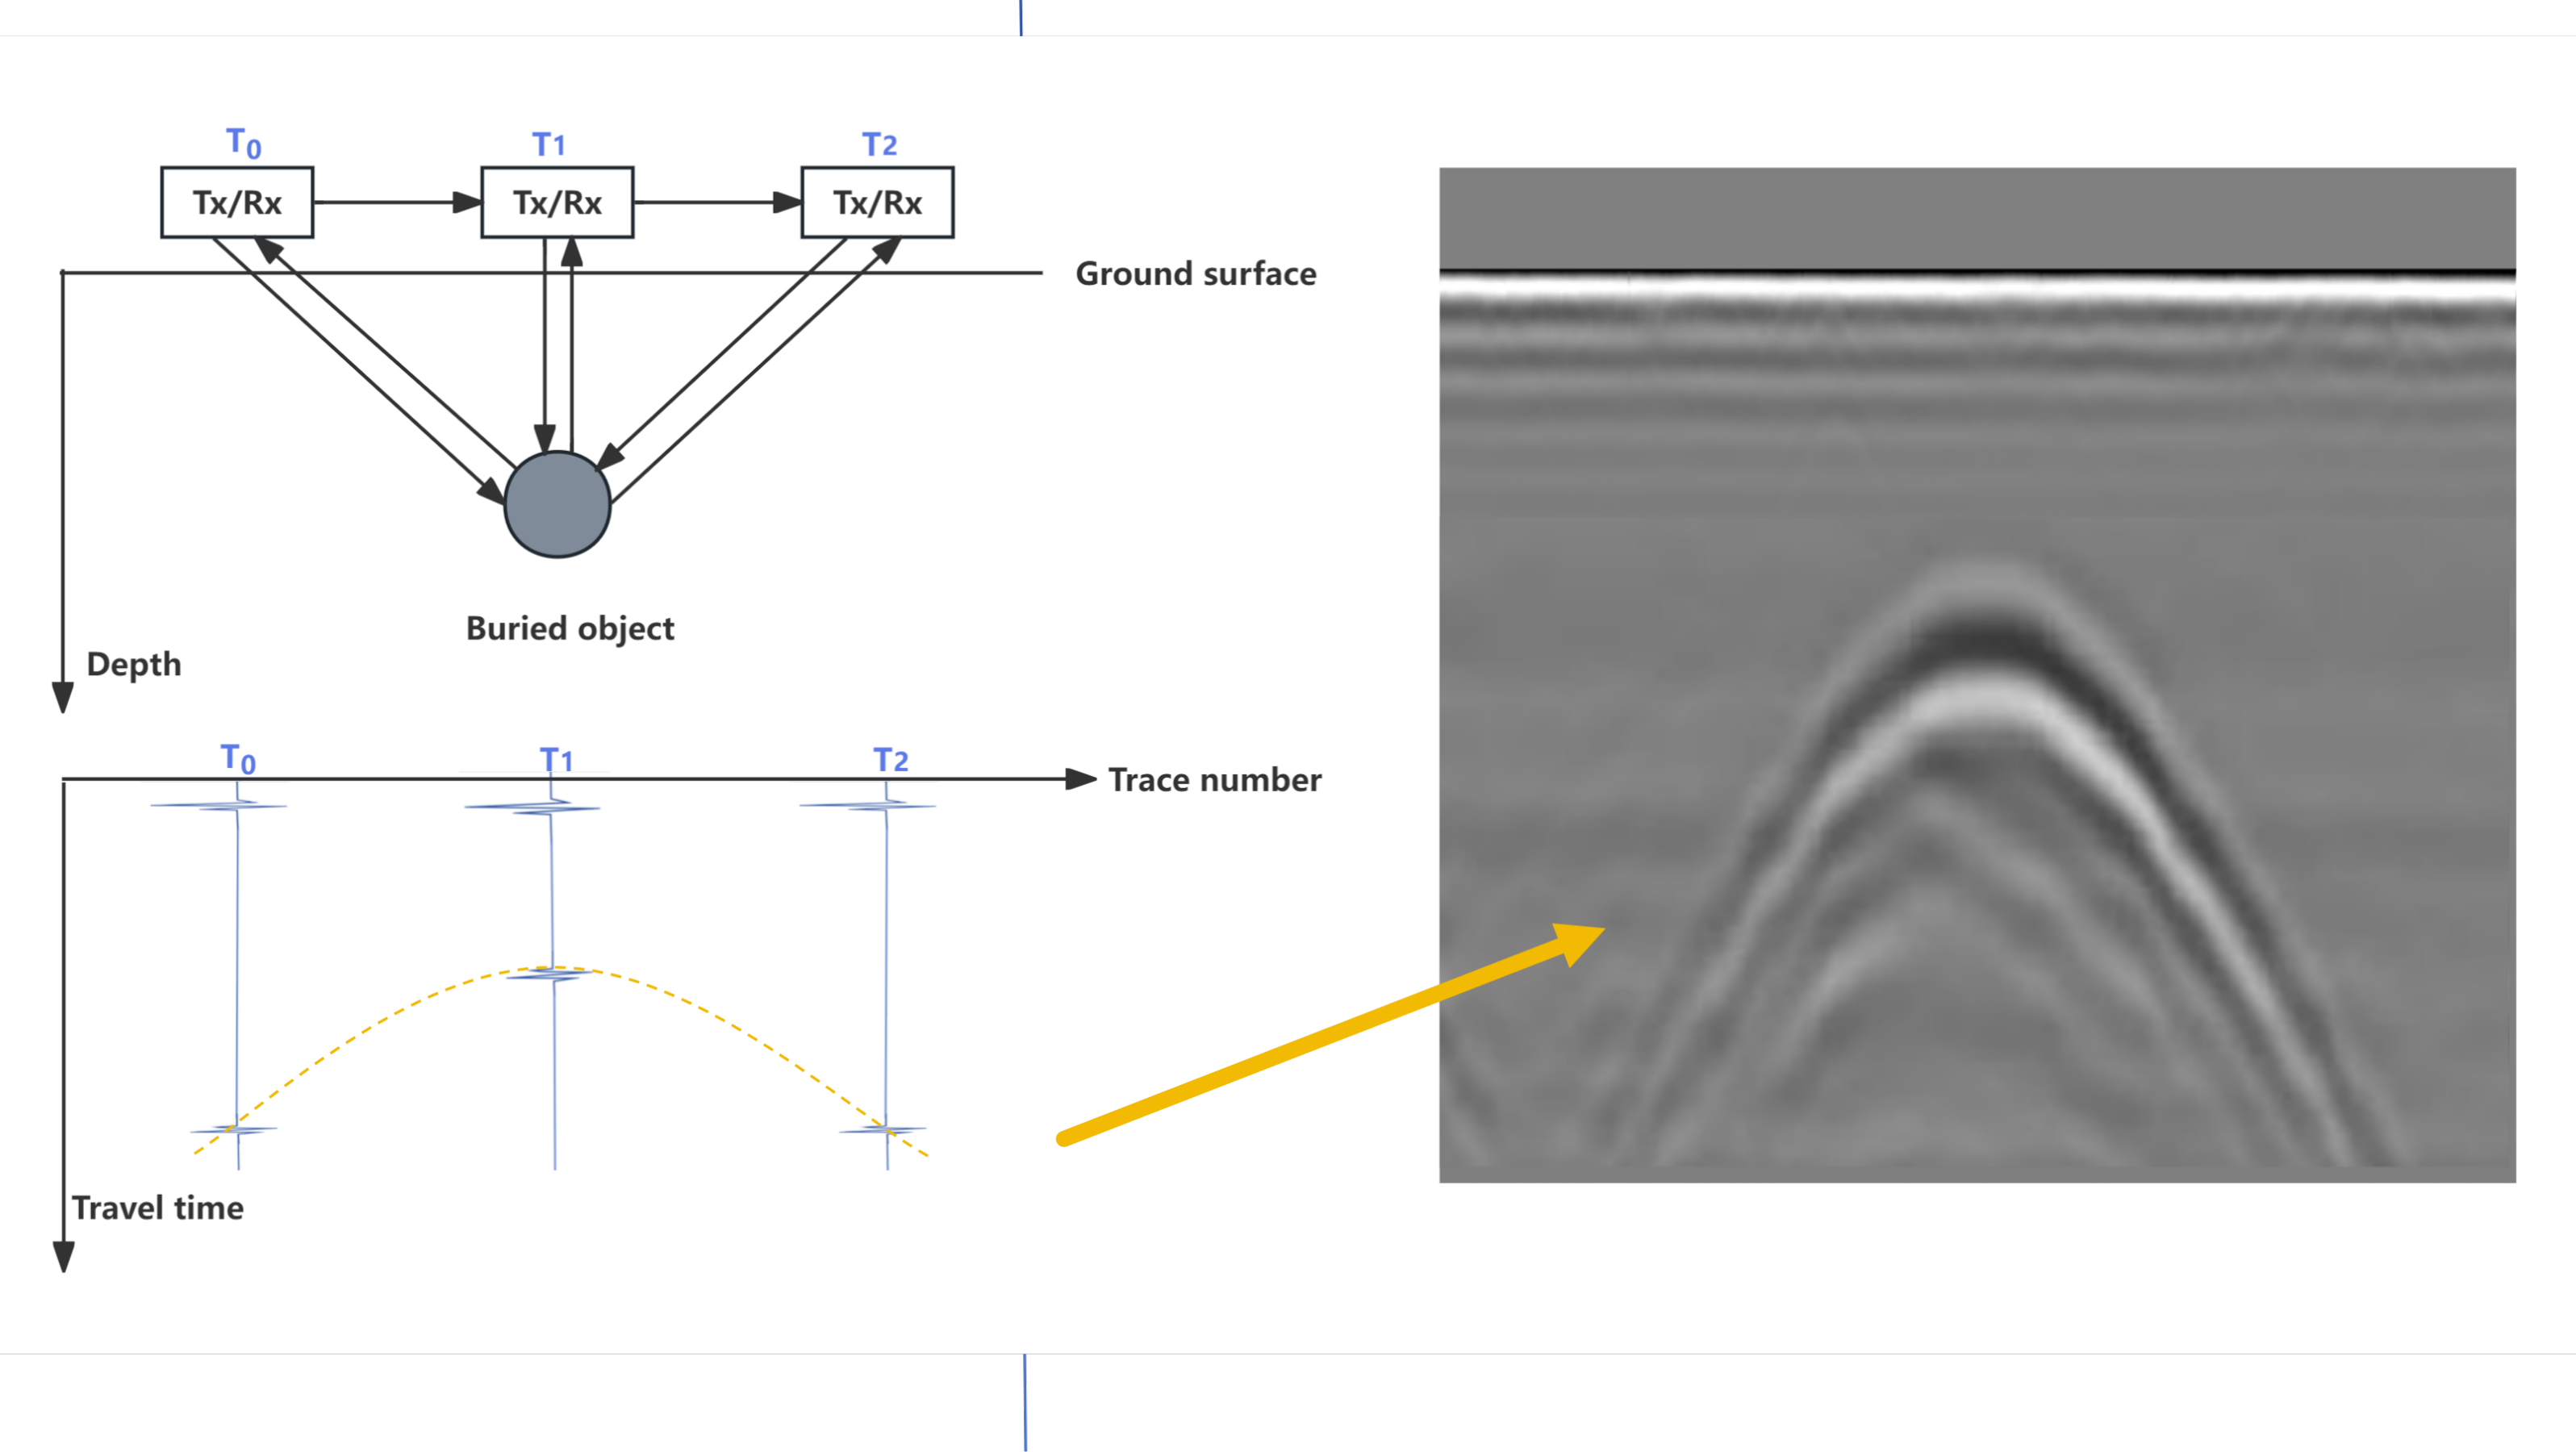
\includegraphics[width=0.9\linewidth, trim={0 40 0 20}, clip]{bscan.png}
\caption{Formation of a GPR B-scan.}
\label{fig:bscan}
\end{figure*}


Fig.~\ref{fig:bscan} shows the GPR data acquisition process: a transmitter-receiver antenna pair traverses along the scanning path,
with measurement points set at regularly spaced time instants $T_0, T_1, T_2, \dots$ (or, alternatively, at uniformly spaced spatial intervals).
At each measurement point,  an electromagnetic pulse emitted by the transmitting antenna is reflected at successive dielectric boundaries~\cite{Solimene10}, such as the air-soil and soil-buried object interfaces. 
A sequence of reflections is then recorded by the receiving antenna, yielding an A-scan trace. Repeating this process at successive measurement points and arranging the resulting A-scans along the survey line produces a two-dimensional radargram, referred to as a B-scan.
Directly above the buried target, the wave travels the shortest path between transmitter and receiver, giving the minimum travel time.
Moving the survey point away from this position lengthens the travel time. 
This progressive increase in travel time produces the familiar hyperbolic signature seen in GPR profiles. 

Despite this well-established principle, 
robust hyperbola detection remains highly challenging in practice, 
owing to weak reflections from deeply buried or small targets, 
strong clutter and noise, and hyperbola deformation or overlap.
%Ground-penetrating radar (GPR) forms a subsurface image by moving a transmitter/receiver (Tx/Rx) antenna along a survey line: at each position $T_0,T_1,T_2,\dots$ it emits an electromagnetic pulse and records the reflected signal as a single trace (an A-scan) of amplitude versus two-way travel time. Stacking consecutive traces side by side yields a B-scan, whose horizontal axis is the trace number (antenna position) and whose vertical axis is travel time, which is monotonically related to depth. Because a compact buried target is illuminated from many antenna positions, its round-trip distance is shortest directly above the object and increases symmetrically to either side, so the target's reflection is imaged as a downward-opening hyperbola (Fig.~\ref{fig:bscan}).

%In GPR B-scan images, buried pipes, cables, and roots typically appear as hyperbolic reflections, making hyperbola detection a prerequisite for target localization, depth estimation, and parameter reconstruction \cite{jin2024gprformer,lei2020cnnlstm,maas2013violahough}. 

Early automated approaches relied on hand-crafted features and analytical fitting, 
screening candidates with neural preprocessing, Viola--Jones,
or histogram of oriented gradients (HOG) features with a support vector machine (SVM) classifier,
and then localizing them via the Hough transform or template/least-squares
fitting~\cite{alnuaimy2000nn,Maas2013Using,lee2014hog,Sagnard2016Template-matching}. 
%Maas and Schmalzl employed the Viola-Jones algorithm to rapidly narrow down candidate regions before applying a hyperbola-specific Hough transform on the reduced search space ~\cite{maas2013violahough}.
%Mertens et al. combined Canny edge detection, analytic hyperbola fitting, and a human-inspired fuzzy-band criterion to handle distorted and irregular hyperbolas, ~\cite{Mertens2015Automated}.
Dou et al. proposed a real-time framework that combines thresholding, column-connection clustering (C3), a lightweight two-feature model, and orthogonal-distance fitting. This framework is designed to handle hyperbolas that are crossing, distorted, or incomplete~\cite{Dou2016Real-Time}.
Such pipelines work in constrained settings but remain computationally expensive, 
sensitive to parameter discretization, and dependent on prior template design or user intervention~\cite{lei2020cnnlstm,pham2018fasterrcnn,Sagnard2016Template-matching,kafedziski2018c3hough}.

%Early methods relied on hand-crafted features and analytical fitting, screening candidates with neural preprocessing, Viola--Jones, or HOG+SVM and then localizing them via the Hough transform or template/least-squares fitting \cite{alnuaimy2000nn,maas2013violahough,lee2014hog,sagnard2016template,dou2017c3}. 
%Such pipelines work in constrained settings but remain computationally expensive, sensitive to parameter discretization, and dependent on prior template design or user intervention \cite{lei2020cnnlstm,pham2018fasterrcnn,sagnard2016template,kafedziski2018c3hough}; later refinements combined edge detection and C3 clustering with Hough fitting to improve robustness \cite{kafedziski2018c3hough,barkataki2023c3}.
Deep learning shifted the field from sliding-window recognition toward end-to-end detection on full B-scans.
Among two-stage detectors, the Faster region-based convolutional neural network (Faster R-CNN) was first trained
on simulated radargrams to offset scarce field labels~\cite{pham2018fasterrcnn}.
Lei et al. subsequently coupled Faster R-CNN with double cluster seeking estimate (DCSE) clustering
and column-based transverse filter points (CTFP) extraction,
which fit the hyperbola after detection to localize buried objects~\cite{lei2019autohyperbola}.
Although accurate, the proposal-then-refine design of such two-stage pipelines makes inference comparatively slow,
so one-stage detectors were favored for real-time deployment.
Liu et al. used the single shot multibox detector (SSD) to identify hyperbolic regions of rebar,
combining migration and binarization to estimate rebar position and depth~\cite{LIU2020103279},
and later applied You Only Look Once version 3 (YOLOv3) with iterative thresholding to pipeline detection,
achieving approximately 12 fps with depth estimation errors within 0.04~m~\cite{liu2022pipeline}.
Subsequent YOLO variants were coupled with explicit curve fitting:
Sun et al. combined YOLOv5s with three-point circle fitting for root localization and diameter estimation~\cite{agronomy13020344},
and Zhu et al. integrated YOLOv7 with keypoint annotation and two-stage curve fitting
to invert pipeline burial depth and radius~\cite{rs15082114}.
YOLO-based detectors excelled in speed, but their local features and non-maximum suppression (NMS) still struggled
with crossing and incomplete hyperbolas, motivating a shift toward transformer-based, end-to-end approaches.
Jin et al.'s GPR-Former used a transformer to directly regress hyperbola parameters,
refined via a symmetry-constrained analytical solution, outperforming both C3 and
transfer-learning-based methods in precision and recall~\cite{jin2024gprformer}.

The field of GPR hyperbola detection has thus seen a shift toward more powerful detection networks
and a broader push from 2D applications toward 3D reconstruction
and multi-sensor fusion~\cite{ma18184400,s26092708}.
Across all these paradigms, however, the hyperbola is still annotated and predicted as an axis-aligned bounding box:
the parametric geometry of the echo enters the pipeline only through a separate post-hoc curve-fitting stage,
and detection performance degrades markedly when labeled data are scarce.
How to exploit the band-like geometry of the hyperbola during detector training itself,
rather than recovering it after detection, remains largely unexplored and motivates the method proposed in this work.


\subsection{Attention Mechanisms in GPR Hyperbola Interpretation}

Attention mechanisms were originally introduced in general image recognition to let a network emphasize informative regions or channels instead of treating all spatial positions and feature channels uniformly: a lightweight sub-network learns a set of weights from the
feature map itself, and these weights rescale the original features so that informative regions or channels are amplified while less relevant ones are suppressed. 

In GPR interpretation, this idea has been adapted so that models respond to hyperbola-relevant structures rather than processing the whole radargram uniformly. Wang et al. first use one network to suppress the direct-wave interference that dominates the upper portion of every B-scan; a second network, built around GPR domain knowledge as prior information, then applies attention together with a feature-fusion step to help the network concentrate on the remaining hyperbola, before it is fitted with a least-squares curve and localized through geometric relations \cite{Wang2025Underground}.

A second line of work instead exploits the fact that the two arms of a hyperbola have a large spatial extent, spreading across many neighbouring measurement positions and the full recording time window -- so that evidence located far apart in the image can still be relevant to identifying the same target. Transformer-style self-attention is naturally suited to this setting, since it lets any two positions in the image establish a direct connection rather than being confined, as convolution is, to a local neighbourhood. GPR-Former adopts this form of attention to regress the hyperbola's geometric parameters, such as its apex position and curvature, directly from the B-scan \cite{jin2024gprformer}.



A third line of work goes further still, embedding the hyperbola's geometry directly into the structure of the attention module itself. To detect the curved, multiply-reflected pattern produced by rebar in concrete, Li et al. let the attention module adapt its receptive field to the target's expected curvature before region proposals are generated, so that the earliest processing stages are already biased toward hyperbola-like structures \cite{li2025rebar}.



Despite this progression toward stronger geometric assumptions, all of these methods share the same limitation: prior knowledge shapes only the network's input or architecture, while the attention weights themselves are still learned indirectly, from a loss defined on the final output. This matters most under the few-shot conditions common in GPR surveys, where the attention map can still drift toward clutter even when the surrounding architecture is built around the target's shape. We take a different approach: we derive an explicit attention target directly from the parametric annotation and use it to supervise the attention branch, imposing the hyperbola's spatial prior on attention directly rather than relying on the architecture alone.


%Attention mechanisms are increasingly embedded into task-specific GPR pipelines so that models respond to hyperbola-relevant structures rather than processing the whole radargram uniformly. Localized hyperbolic attention enhances hyperbolic wave features and suppresses clutter to improve downstream imaging of target pipelines \cite{liu2025hyperbolic}, while a dual-cascade network first removes direct-wave interference and then applies attention with feature fusion to raise hyperbola detection accuracy before geometric localization \cite{wang2025underground}. Because hyperbolic reflections extend across neighbouring traces and the full time window, transformer-style self-attention is also used to model the long-range dependencies that convolution captures less efficiently: GPR-Former regresses hyperbola parameters directly from B-scans and refines them with a symmetry constraint \cite{jin2024gprformer}, and GPR-TransUNet introduces self-attention into a TransUNet-style regression framework for the same reason \cite{ge2024gprtransunet}.

%More recent designs tailor attention specifically to hyperbolic geometry and apex-localization objectives that are closely aligned with our study. A rebar-recognition model emphasizes hyperbolic features with deformable attention and a hyperbolic attention transformer before proposal generation \cite{li2025rebar}, a lightweight dual-task keypoint detector couples attention-enhanced features with keypoint regression for precise vertex localization \cite{hou2025endtoend}, and a state-space detector for arbitrarily long B-scans targets hyperbola vertex estimation directly \cite{lan2024statespace}. The clear trend is a shift from generic channel or spatial reweighting toward physically informed designs that encode hyperbolic structure and apex localization, while traditional fitting-based pipelines remain relevant for their geometric interpretability \cite{lei2019autohyperbola}. This motivates our approach: instead of localizing the echo through rectangular proxies or post-hoc curve fitting, we represent the hyperbola by its strip-like, symmetric, parametric shape, so that both annotation and learning are aligned with the geometry of the target.


\subsection{Annotation of hyperbolic reflections}
Training a detection model requires large quantities of manually annotated images,
and a variety of general-purpose annotation tools have been developed to meet this need.
Early systems such as LabelMe enabled collaborative image labelling at scale \cite{russell2008labelme},
and the annotation pipelines behind large-scale benchmarks such as Microsoft common objects in context (MS-COCO)
further standardized this process \cite{lin2014coco}.
Building on these efforts, widely used open-source tools such as LabelImg \cite{tzutalin2015labelimg}
and the computer vision annotation tool (CVAT) \cite{cvat} offer interactive interfaces for a common set of
geometric shapes: axis-aligned rectangles, polygons, key points, and pixel-wise masks.
Being generic and domain-agnostic, these shapes are precisely 
what makes such tools broadly applicable across natural-image tasks.

In GPR interpretation, hyperbolic reflections are typically annotated with these same general-purpose shapes.
Bounding boxes remain the most common choice for subsurface targets in B-scans~\cite{besaw2015deep},
whereas a growing body of work instead marks the apex of each hyperbola as a keypoint and treats it as
the localization target~\cite{hou2025endtoend,lan2024statespace}; segmentation masks have also been used to
delineate the hyperbola or its apex region more tightly~\cite{hou2021msrcnn}.
Each of these schemes, however, captures only part of the geometry: a bounding box records merely the extent
of the echo, a single keypoint pins down only the apex while discarding the opening and curvature of the curve,
and segmentation masks demand dense per-instance labelling yet still do not expose the underlying hyperbola parameters.
None of them aligns with the parametric, band-shaped nature of the hyperbola or offers direct geometric supervision.
This mismatch motivates the dedicated annotation tool proposed in this work, which allows annotators to place and
adjust a parametric hyperbola band through a few interpretable controls, and to export both the shape parameters
and the derived bounding box.


\section{Proposed method}
\subsection{Hyperbola-Band Annotation}
%我们设计了一个 双曲线带状目标的可视化标注工具。该工具的使用界面如图所示。
%首先，选择图片的文件夹，然后会自动加载其中的图片
%然后下方左侧会显示原图，右侧会显示标注后的图片。
%在左图单击的点为双曲线的顶点位置，右侧可以调节各个参数。
%我们设定了5个参数。分别是双曲线顶点的横纵坐标，渐近线斜率slope，水平跨度span和带状厚度thickness。斜率是唯一的形状参数，编码波速；顶点深度即竖直半轴a，b=y_vertex/slope。
%点 Add as New Annotation 把当前参数作为一个新标注加入当前图片，并且可以在同一个图中添加多个标注。
%我们的标注通过json格式保存
We designed \textbf{HBAT}, a visual annotation tool for hyperbola-band targets that supports parametric hyperbola annotation with automatic bounding-box generation. Its user interface is illustrated in Fig.~\ref{fig:The HBAT annotation interface}.

First, the user selects an image folder, and the tool automatically loads all images within it.
The original image is displayed on the lower-left panel, while the annotated image is shown on the right.
A mouse click on the original image marks the vertex position of the hyperbola, and five adjustable parameters are provided on the right panel.

The five parameters are defined as follows: the horizontal coordinate $x_{\mathrm{vertex}}$ and 
vertical coordinate $y_{\mathrm{vertex}}$ of the hyperbola vertex, the slope $s$, the horizontal span, and the ribbon thickness.
Among these, the slope $s$ is the only parameter that governs the shape of the curve. 
Once the vertex is placed, a single slope value fully fixes the openness of the two arms, 
so a larger slope yields a narrower and sharper hyperbola and a smaller slope yields a flatter one.
The centreline of the downward-opening band is
\begin{equation}
y_c(x) = y_{\mathrm{vertex}}\sqrt{1 + \left(\frac{s\,(x - x_{\mathrm{vertex}})}{y_{\mathrm{vertex}}}\right)^2},
\end{equation}
and the band is the vertical ribbon of all points $(x,y)$ satisfying $|y - y_c(x)| \le \mathrm{thickness}/2$, 
where the span sets the horizontal extent over which the two arms are drawn.
By clicking the \emph{Add as New Annotation} button, 
the current parameter configuration is saved as a new annotation for the active image, 
and multiple annotations can be added to a single image.

All annotations are stored in JSON format with the following structure:
\begin{verbatim}
{
  "line2888_0-100_jpg.rf.ce38dc3799
  2454823c8dea9e0f814ac5.jpg": [
    {
      "label": "hyperbola",
      "x_vertex": 315.4,
      "y_vertex": 241.5,
      "slope": 3.09,
      "span": 387.9,
      "thickness": 115.8
    }]
}
\end{verbatim}

Here, the top-level key denotes the image filename, 
and each list entry stores one annotated hyperbola band as its parameters and their corresponding values.


\begin{figure*}
\centering
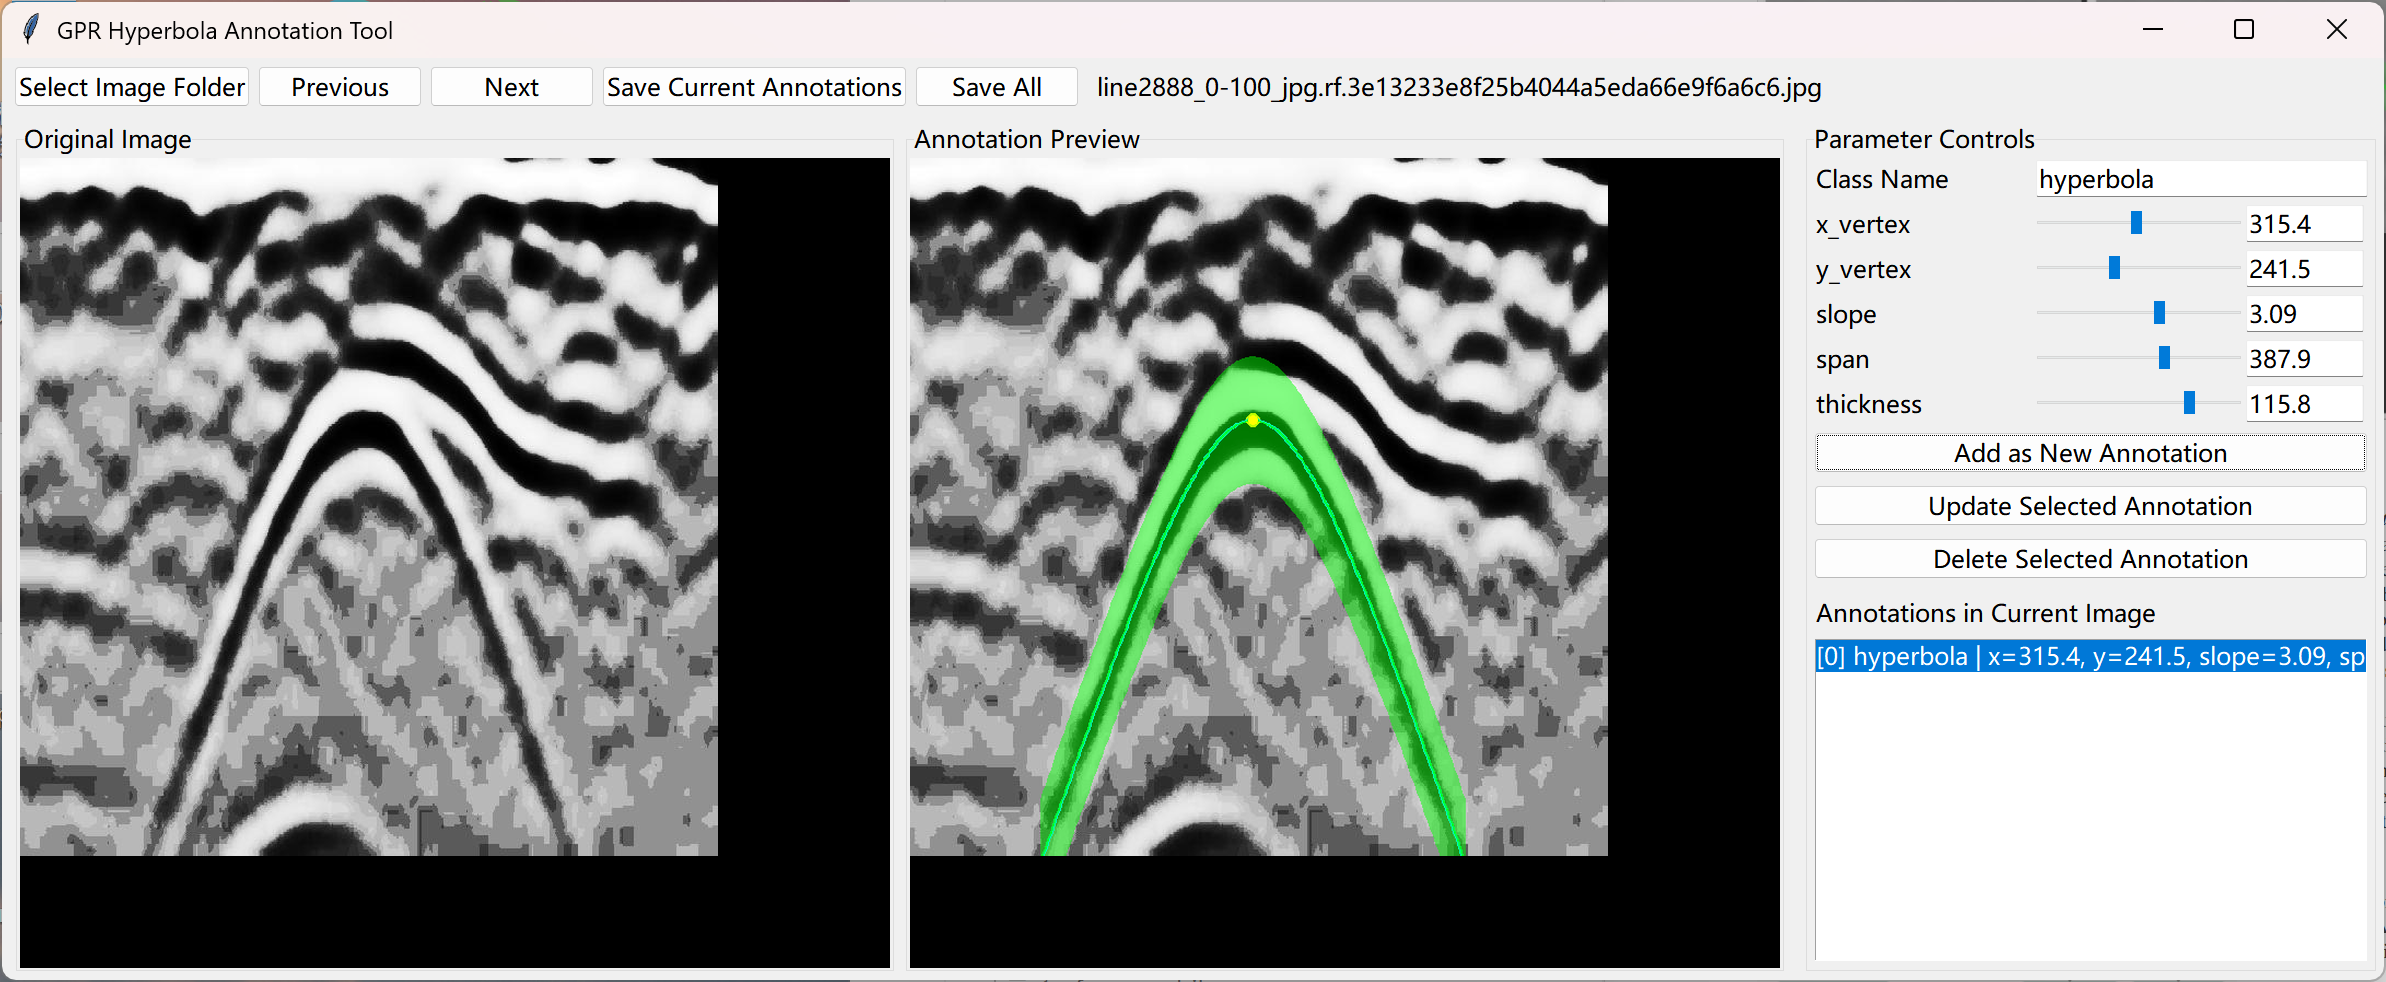
\includegraphics[width=1\linewidth]{annotationtool.png}
\caption{The HBAT annotation interface}
\label{fig:The HBAT annotation interface}
\end{figure*}

%在标注完双曲线带之后，对应的常见形式的boudinbg box形式的标注可以有双曲线的边界直接导出。
%图展示了例子，分别是原图，标注的双曲线带和对应的bouding box形式。
After the hyperbola band is annotated, the conventional bounding-box annotation can be directly derived from the boundary of the band. 
Fig.~\ref{fig:dataset_samples} shows an example, presenting the raw image, the annotated hyperbola band, and the corresponding bounding-box form.
\begin{figure}[]
    \centering
  \subfloat[\footnotesize Raw image.]{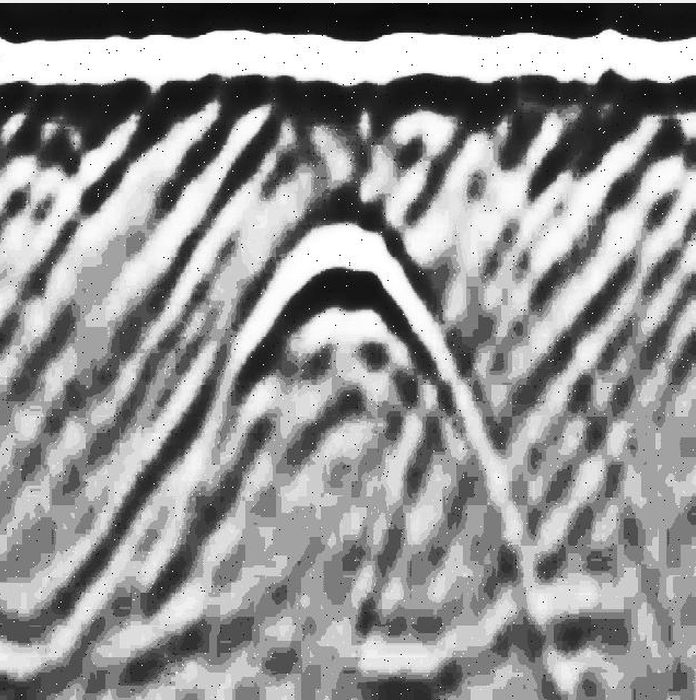
\includegraphics[width=0.31\linewidth]{example-yuantu.png}}
  \hfill
  \subfloat[\footnotesize Annotated hyperbola band.]{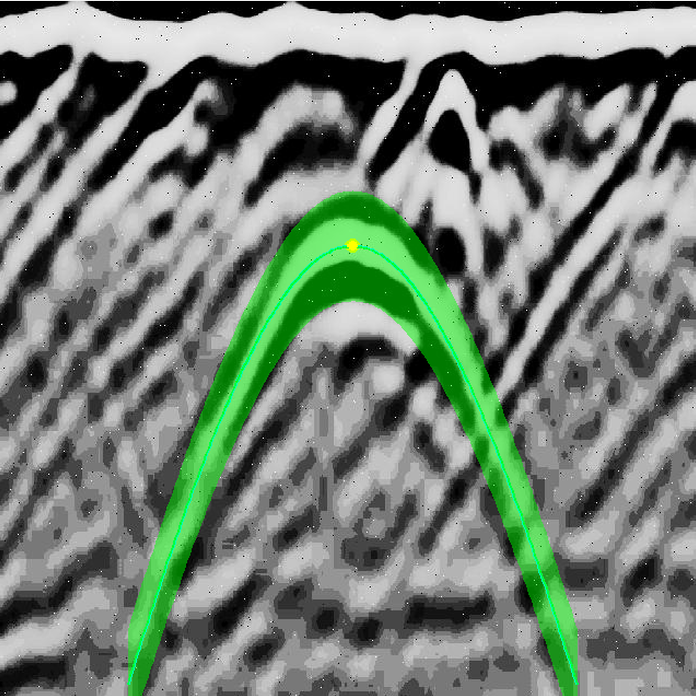
\includegraphics[width=0.31\linewidth]{example-shuangquxian.png}}
  \hfill
  \subfloat[\footnotesize Derived bounding box.]{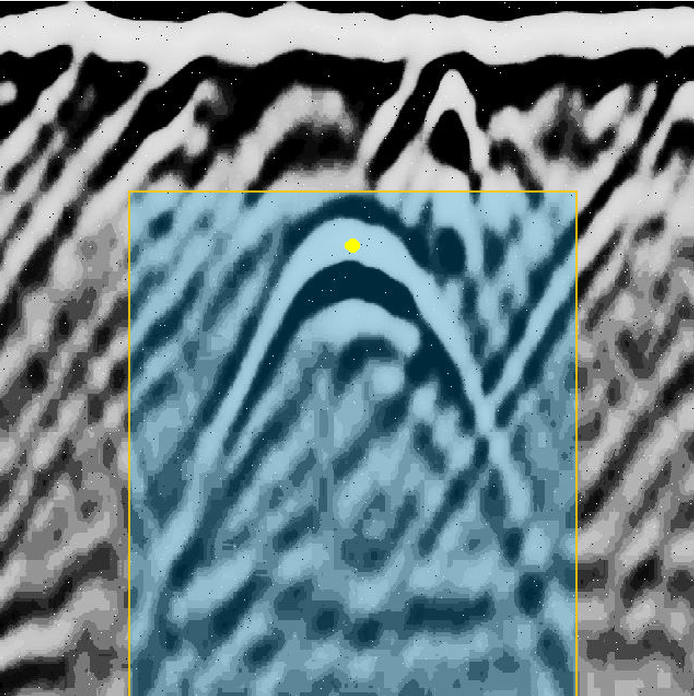
\includegraphics[width=0.31\linewidth]{example-bbox.png}}
  \caption{Example of a hyperbola sample: the raw image, the annotated hyperbola band, and the bounding box derived from the band boundary.}
  \label{fig:dataset_samples}
\end{figure}



\subsection{Hyperbola-attention neural network}
%网络以单通道灰度 B-scan 图像为输入,输出图像中各双曲线带的矩形边界框。
%区别于已有方法,本文在主干网络内部引入一条受双曲线条带掩膜显式监督的注意力分支,并通过通道拼接将其注入瓶颈特征,从而引导网络更加关注双曲线从而提升检测性能。
%网络的示意图如图所示。
The network takes a single-channel grayscale B-scan image as input and outputs a rectangular bounding box for each hyperbolic signature in the image.
Unlike existing methods, we introduce within the backbone an attention branch that is explicitly supervised by a hyperbola-band mask, 
and inject it into the bottleneck features via channel-wise concatenation, thereby guiding the network to focus on the hyperbolas and improving detection performance.
A schematic of the network is shown in Fig.~\ref{fig:framework}.

\begin{figure*}
\centering
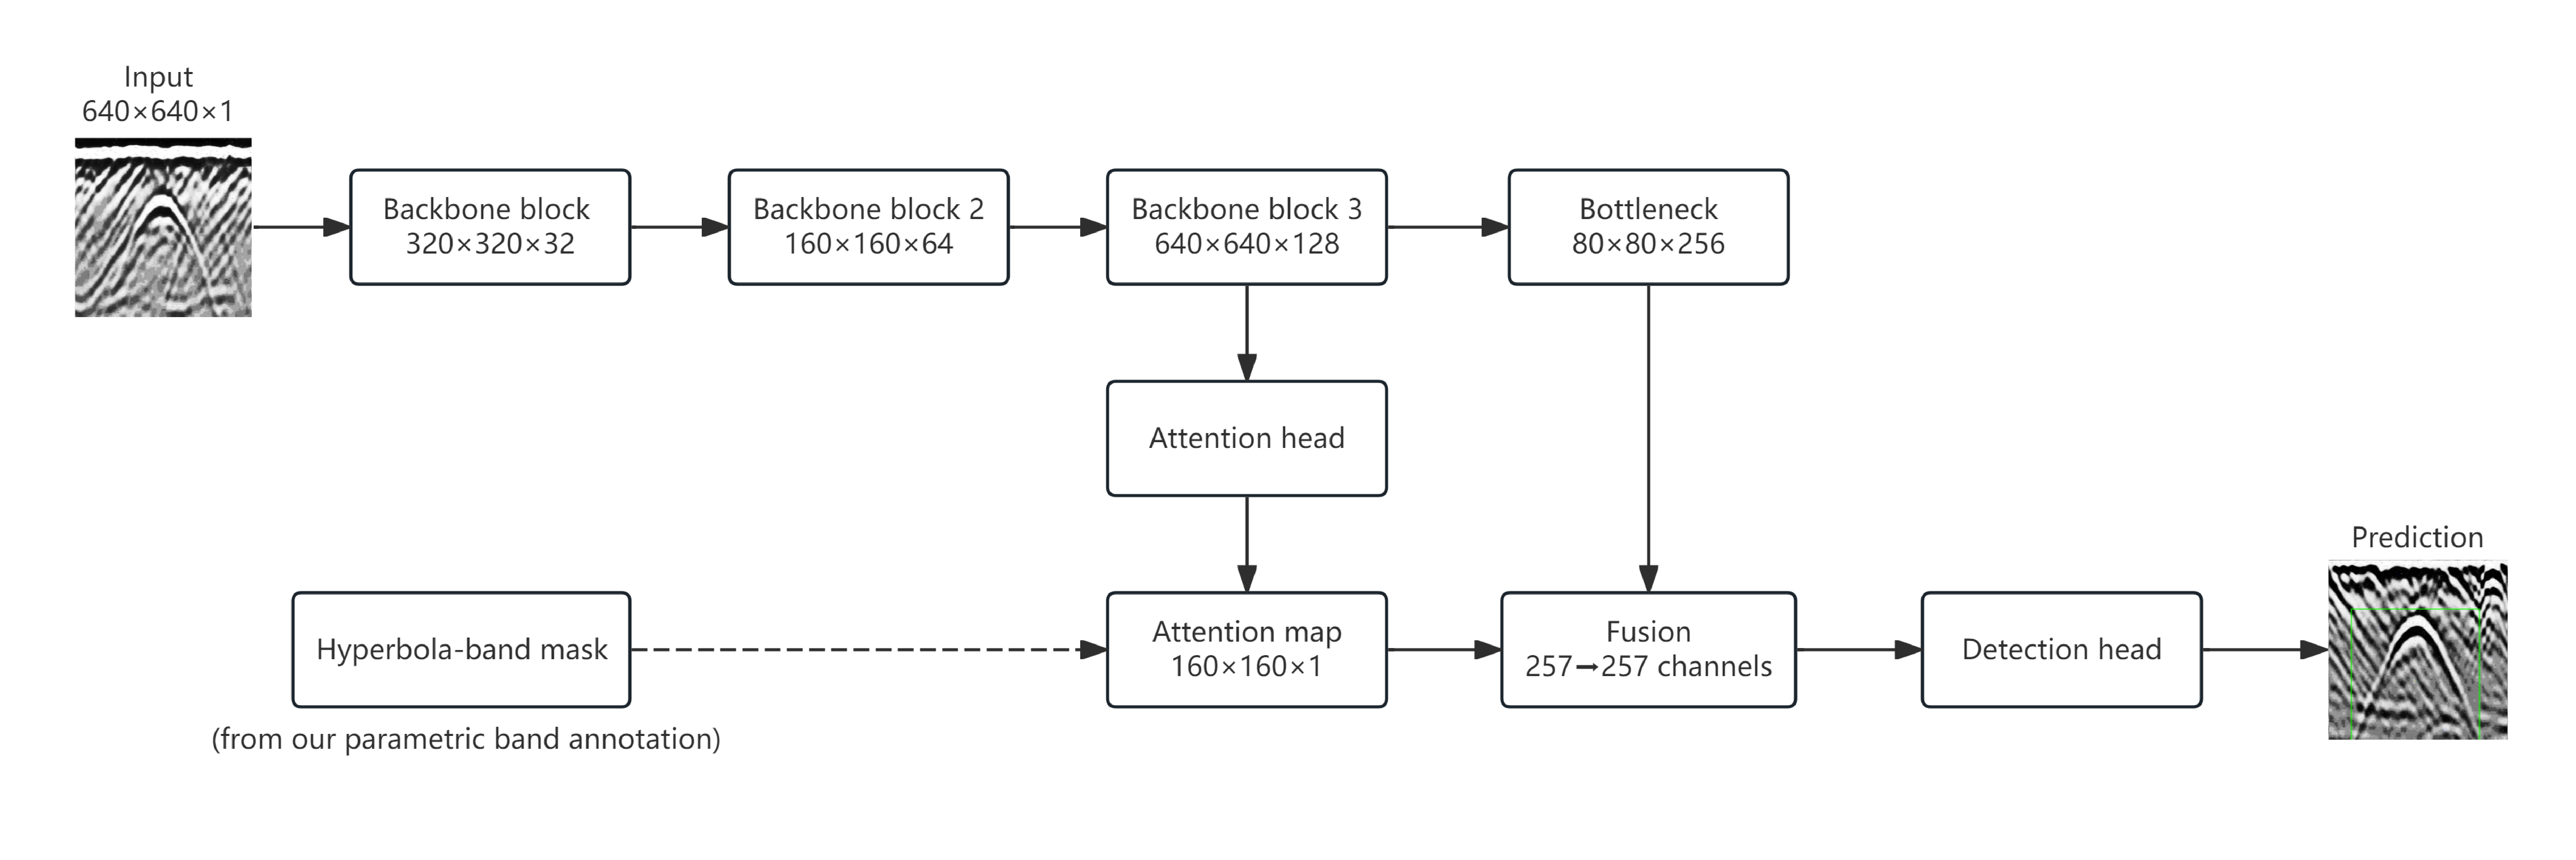
\includegraphics[width=1\linewidth]{framework.pdf}
\caption{Overview of the proposed network.}
\label{fig:framework}
\end{figure*}

The backbone consists of three down-sampling stages followed by a bottleneck layer; 
each stage comprises two $3\times3$ convolutions, 
each followed by batch normalization and ReLU, 
together with a subsequent $2\times2$ max-pooling operation 
that doubles the channel depth while halving the spatial resolution.
Starting from the $1\times640^2$ input, 
the three stages produce feature maps $f_1$ of size $32\times320^2$, $f_2$ of size $64\times160^2$, 
and $f_3$ of size $128\times160^2$, which are further reduced to the bottleneck feature $F_b$ of size $256\times80^2$.
The attention branch takes $f_3$ as input rather than the bottleneck feature $F_b$, 
as $f_3$ retains a higher spatial resolution that is better suited to precise localization.


% 监督注意力分支为本文方法的核心。轻量注意力头 $g_a(\cdot)$ 由一层 $3\times3$ 卷积、批归一化与 ReLU 及一层 $1\times1$ 卷积构成,将 $f_3$ 映射为单通道注意力图,并经 sigmoid 激活得到 $A$。作为监督真值,本文依据标注的双曲线几何参数光栅化生成条带掩膜 $B$。随后,采用二值交叉熵与 Dice 联合损失 $\mathcal{L}_{\mathrm{att}} = \mathcal{L}_{\mathrm{bce}} + \mathcal{L}_{\mathrm{dice}}$ 逐像素约束 $A$ 逼近 $B$。其中,二值交叉熵可理解为对每个像素单独做"是/否属于双曲线带"的二分类判断,并逐一惩罚判断错误的像素;Dice 项则直接衡量预测区域与真值区域的整体重叠程度,重叠越高损失越小。二者互补:前者保证逐像素的判别精度,后者保证区域级的形状一致性,并可缓解条带区域相对图像背景占比过小所带来的类别不平衡问题。

The supervised attention branch is the central component of the proposed method. 
A lightweight head $g_a(\cdot)$, consisting of a $3\times3$ convolution with batch normalization 
and ReLU followed by a $1\times1$ convolution, maps $f_3$ to a single-channel logit 
that is passed through a sigmoid to yield the attention map $A\in[0,1]^{H\times W}$,
whose entry $A_i$ is the predicted probability that pixel $i$ belongs to the hyperbola band.
The supervisory target $B\in\{0,1\}^{H\times W}$ is a binary band mask rasterized from the annotated hyperbola geometry at the same resolution.
The attention map $A$ is then driven to approximate $B$ by a loss that combines a binary cross-entropy term and a Dice term, both computed between $A$ and $B$ over the $N=HW$ pixels,
\begin{equation}
\mathcal{L}_{\mathrm{att}} = \mathcal{L}_{\mathrm{bce}} + \mathcal{L}_{\mathrm{dice}},
\end{equation}
\begin{equation}
\mathcal{L}_{\mathrm{bce}} = -\frac{1}{N}\sum_{i=1}^{N}\Big[B_i\log A_i + (1-B_i)\log(1-A_i)\Big],
\end{equation}
\begin{equation}
\mathcal{L}_{\mathrm{dice}} = 1 - \frac{2\sum_{i=1}^{N} A_i B_i}{\sum_{i=1}^{N} A_i + \sum_{i=1}^{N} B_i + \epsilon},
\end{equation}
where $\epsilon=10^{-6}$ is a small constant added to the denominator to avoid division by zero.
The cross-entropy term performs an independent per-pixel classification, penalizing each pixel that is misclassified as belonging to, or not belonging to, the hyperbola band.
The Dice term instead measures the overall overlap between $A$ and $B$, with the loss decreasing as the overlap increases.
The two terms are complementary: the former enforces pixel-level accuracy, 
while the latter enforces region-level shape consistency 
and helps mitigate the class imbalance caused by the band occupying only a small fraction of the image.

\paragraph{Attention-guided feature fusion}
The attention map $A$ is passed through a sigmoid and downsampled by a factor of two via average pooling 
to align with the bottleneck resolution, yielding $\tilde{A}$. 
It is then concatenated with $F_b$ along the channel dimension 
and compressed back to 256 channels by a $1\times1$ convolution with batch normalization and ReLU, 
producing the fused feature $\hat{F}$. 
This operation injects the spatial prior of the hyperbola band into the feature representation passed to the detection head.

\paragraph{Detection head and prediction}
The detection head follows a YOLO-style dense prediction paradigm, 
producing three parallel outputs over an $80\times80$ grid at stride 8: 
objectness (1 channel), box size (2 channels), and sub-pixel center offset (2 channels). 
During inference, grid cells whose sigmoid-activated objectness exceeds a threshold $\tau$ are decoded into bounding boxes, 
and redundant detections are removed by box-level intersection-over-union (IoU)-based NMS.
Let $\mathcal{P}$ denote the set of positive cells, namely the grid cells that contain an object center, and $\mathcal{N}$ the remaining background cells.
The objectness map is supervised by a class-balanced binary cross-entropy over the hard targets $p_j$, which equal $1$ at positive cells and $0$ elsewhere,
\begin{equation}
\mathcal{L}_{\mathrm{obj}} = \frac{1}{|\mathcal{P}|}\sum_{j\in\mathcal{P}} \mathrm{BCE}(\hat{o}_j, 1)
+ \frac{\lambda_{\mathrm{noobj}}}{|\mathcal{N}|}\sum_{j\in\mathcal{N}} \mathrm{BCE}(\hat{o}_j, 0),
\end{equation}
where $\hat{o}_j$ is the predicted objectness logit at cell $j$ and $\lambda_{\mathrm{noobj}}=0.5$ down-weights the dominant background cells.
The box-size and center-offset branches are regressed only at the positive cells with an $\ell_1$ loss,
\begin{equation}
\mathcal{L}_{\mathrm{size}} = \frac{1}{|\mathcal{P}|}\sum_{j\in\mathcal{P}} \lVert \hat{s}_j - s_j \rVert_1,
\qquad
\mathcal{L}_{\mathrm{off}} = \frac{1}{|\mathcal{P}|}\sum_{j\in\mathcal{P}} \lVert \hat{\delta}_j - \delta_j \rVert_1,
\end{equation}
where $s_j$ and $\delta_j$ are the ground-truth box size and sub-pixel center offset and $\hat{s}_j$, $\hat{\delta}_j$ their predictions.
The detection loss is the sum of the three terms,
\begin{equation}
\mathcal{L}_{\mathrm{det}} = \mathcal{L}_{\mathrm{obj}} + \mathcal{L}_{\mathrm{size}} + \mathcal{L}_{\mathrm{off}},
\end{equation}
and the overall training objective combines it with the attention supervision loss introduced above,
\begin{equation}
\mathcal{L} = \mathcal{L}_{\mathrm{det}} + \lambda\, \mathcal{L}_{\mathrm{att}},
\end{equation}
where $\lambda$ controls the relative weight of the attention supervision. All terms are optimized jointly in a single end-to-end training pass.


\section{Result and evaluation}
\subsection{Implementation Details}
\label{sec:impl}
%本文的数据集是universe.roboflow上的数据集。一共有318张图片，所有的实验都在十个随机种子下进行，按比例划分训练数据集 剩下的比例是训练数据集。
%测试结果是10次结果的平均并附上了std。
The dataset used in this study is a publicly available GPR dataset, 
comprising 318 B-scan images in total.
For each experiment, the images are randomly split into a training set according to a specified ratio, 
with the remaining images used as the test set. 
All experiments are conducted under ten random seeds, 
and the reported results are averaged over the ten runs,
with the corresponding standard deviations provided.
For evaluation, a predicted box is counted as a true positive if its IoU
with a ground-truth box is at least 0.5, and each ground-truth box can be matched at most once;
precision, recall, and F1-score are then computed accordingly.

All experiments are implemented in PyTorch and run on a single NVIDIA GeForce RTX 5060 Ti GPU (8 GB)
with an AMD Ryzen 7 9800X3D CPU.
The main training settings are summarized in Table~\ref{tab:impl}.

\begin{table}[]
\caption{Training Settings}
\label{tab:impl}
\centering
\begin{tabular}{ll}
\toprule
Item & Setting \\
\midrule
Optimizer & Adam \\
Learning rate & $5\times10^{-4}$ \\
Batch size & 8 \\
Training epochs & 100 \\
Mixed precision & bfloat16 \\
\bottomrule
\end{tabular}
\end{table}

\subsection{Detection performance}
% 表展示了不同训练数据比例下的检测性能。可以看出，在所有训练数据比例下，本文方法均优于基线方法。
% 在训练数据比例为0.7时，本文方法的F1-score提升最为显著，达到了0.84，相比基线方法的0.68有了明显的提升。
% 并且稳定性也有了明显的提升，标准差从0.21下降到了0.03。
% 增益主要来自于recall的提升，这是因为注意力约束引导网络更加关注双曲线带区域，从而减少了漏检的情况。
% 证明了我们方法的有效性。

% 但是我们也可以看到在训练数据比例为0.9时，检测性能无明显提升并且稳定性较差。
% 这可能时因为测试数据集样本量较少，导致评估结果不稳定。

% 以上结果的是在lambda=0.7的情况下得到的。我们还进行了lambda参数敏感性分析在后文中说明。
Table~\ref{tab:bbox_results} reports the detection performance under different training-data ratios. 
As can be observed, the proposed method consistently outperforms the baseline across all training-data ratios. 
The improvement in F1-score is most pronounced at a training-data ratio of 0.7, 
where our method achieves 0.84 compared with 0.68 for the baseline. 
The training stability is also notably enhanced, with the standard deviation decreasing from 0.21 to 0.03. 
This gain is primarily attributed to the improvement in recall, 
as the attention constraint guides the network to focus on the hyperbola-band regions and thereby reduces missed detections, 
which demonstrates the effectiveness of the proposed method.

Nevertheless, at a training-data ratio of 0.9, 
no significant improvement is observed and the stability is relatively poor. 
This is presumably due to the limited number of samples in the test set, 
which leads to unstable evaluation results. 

It should be noted that the above results are obtained with $\lambda=0.7$; 
a sensitivity analysis of the parameter $\lambda$ is further presented in Section~\ref{lambda}.

\begin{table*}[]
\centering
\caption{Detection performance (mean $\pm$ std over 10 seeds) at different
training-data ratios. ``Ours'' uses the attention constraint with
$\lambda_{\mathrm{att}}=0.7$. The best F1 per row is shown in \textbf{bold}.}
\label{tab:bbox_results}
\setlength{\tabcolsep}{4pt}
\renewcommand{\arraystretch}{1.2}
\begin{tabular}{c ccc ccc}
\toprule
\multirow{2}{*}{Training ratio} &
\multicolumn{3}{c}{Baseline} &
\multicolumn{3}{c}{Ours} \\
\cmidrule(lr){2-4} \cmidrule(lr){5-7}
 & Precision & Recall & F1-score
 & Precision & Recall & F1-score \\
\midrule
0.5 & 0.81\,$\pm$\,0.19 & 0.43\,$\pm$\,0.09 & 0.53\,$\pm$\,0.07
    & 0.86\,$\pm$\,0.08 & 0.49\,$\pm$\,0.07 & \textbf{0.62\,$\pm$\,0.06} \\
0.6 & 0.71\,$\pm$\,0.20 & 0.56\,$\pm$\,0.08 & 0.60\,$\pm$\,0.10
    & 0.75\,$\pm$\,0.24 & 0.65\,$\pm$\,0.06 & \textbf{0.66\,$\pm$\,0.12} \\
0.7 & 0.75\,$\pm$\,0.29 & 0.68\,$\pm$\,0.10 & 0.68\,$\pm$\,0.20
    & 0.91\,$\pm$\,0.08 & 0.78\,$\pm$\,0.04 & \textbf{0.84\,$\pm$\,0.03} \\
0.8 & 0.84\,$\pm$\,0.21 & 0.82\,$\pm$\,0.07 & 0.81\,$\pm$\,0.15
    & 0.91\,$\pm$\,0.12 & 0.88\,$\pm$\,0.04 & \textbf{0.89\,$\pm$\,0.07} \\
0.9 & 0.87\,$\pm$\,0.23 & 0.90\,$\pm$\,0.06 & 0.87\,$\pm$\,0.16
    & 0.85\,$\pm$\,0.21 & 0.93\,$\pm$\,0.04 & \textbf{0.87\,$\pm$\,0.16} \\
\bottomrule
\end{tabular}\\
Note: At ratio 0.9, Ours shows lower precision but higher recall than the baseline; \\these opposing shifts happen to offset, yielding the same F1 score.
\end{table*}

\subsection{Visualization of attention maps}
%0-88可能可以0630的结果
%第一行  标注 矩形标注  无注意力的结果   无注意力的注意力
%第二行   双曲线带 标注  有注意力的结果   有注意力的注意力
%可能第一列的标注不需要？
To visualize where the network attends, we adopt gradient-weighted class activation mapping (Grad-CAM)~\cite{selvaraju2017gradcam},
a widely used method for interpreting the predictions of convolutional networks.
Intuitively, it produces a heatmap over the input image in which brighter regions are the ones that
contribute most to the network's decision, 
so we can directly see which parts of the image the model relies on when making a detection. 
Fig.~\ref{fig:attn_vis} shows a representative sample, 
where we use Grad-CAM to visualize the regions that the network relies on. 
The top row corresponds to the baseline without attention supervision, 
and the bottom row to our method; 
the left column shows the detection results and the right column the corresponding Grad-CAM maps. 
For the baseline, the attention is mostly scattered over the background, 
so the model fails to focus on the hyperbola band and does not detect it. 
In contrast, with the explicit supervision on the hyperbola band, 
our method attends not only to a few background curves but also to the hyperbola band itself, 
clearly capturing the overall hyperbolic structure and thus producing a correct detection. 
This comparison demonstrates the effectiveness of the proposed attention supervision.
\begin{figure}[]
    \centering
  \subfloat[Baseline detection.]{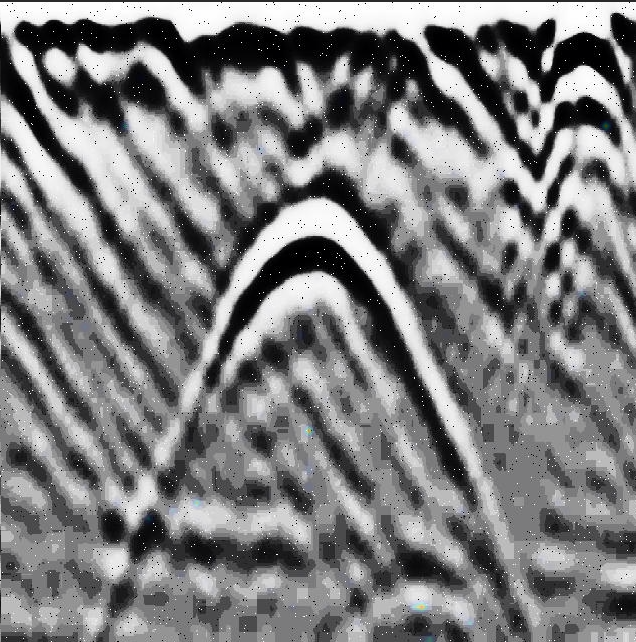
\includegraphics[width=0.48\linewidth]{baseline-result.png}}
  \hfill
  \subfloat[Baseline attention.]{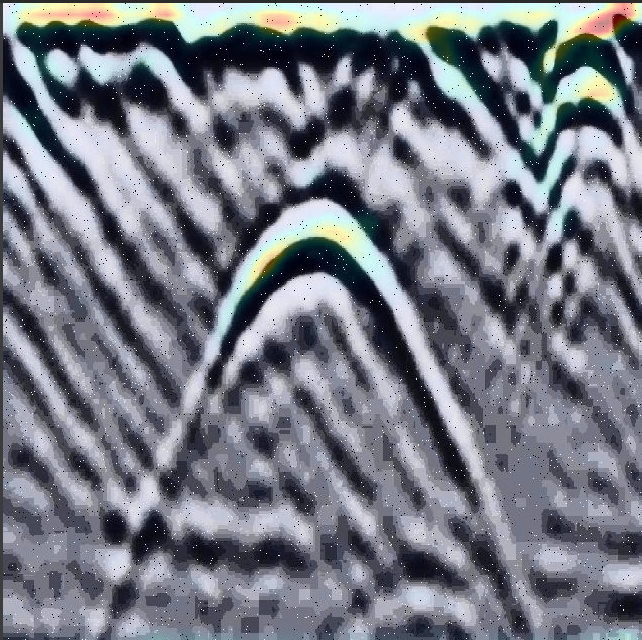
\includegraphics[width=0.48\linewidth]{baseline-attention.png}}
  \\
  \subfloat[Our detection.]{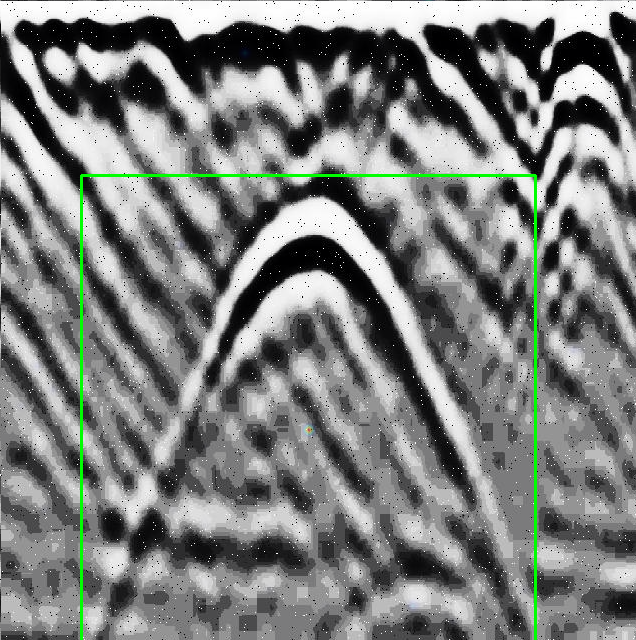
\includegraphics[width=0.48\linewidth]{our-result.png}}
  \hfill
  \subfloat[Our attention.]{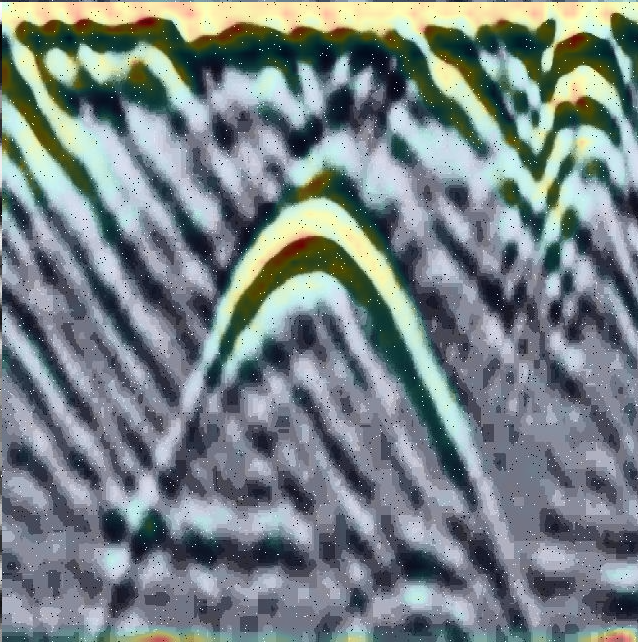
\includegraphics[width=0.48\linewidth]{ours-attention.png}}
  \caption{Visualization of attention maps.}
  \label{fig:attn_vis}
\end{figure}

%加上可视化的比较 他漏掉了什么 我们对了什么
\subsection{Comparison of Detection Performance with Different Attention Modules}
%和其他注意力机制比较  ok
%表~\ref{tab:attention_comparison} 将本文方法与若干已在探地雷达、SAR 及遥感识别中得到应用的代表性注意力模块进行了对比:Pan et al. 采用通道注意力 SE,N. Wang et al. 采用通道—空间注意力 CBAM,Z. Wang et al. 采用非局部注意力 Non-local,Shen et al. 采用坐标注意力 CA。为公平比较,我们将上述注意力模块在相同骨干网络的同一位置进行复现,并在本文双曲线数据集上以完全一致的训练与评估设置进行实验,表中所有结果均由本文复现得到。本文方法在精确率、召回率和 F1 上均取得最优,F1 达到 0.89,较次优方法提升约 9%。现有模块普遍难以兼顾精确率与召回率,而本文方法同时获得最高的精确率与召回率,且 F1 标准差最低,兼具更高的检测精度与稳定性。究其原因,SE、CBAM、Non-local 与 CA 均属于自学习的注意力机制,仅依据特征自身对通道或空间进行重加权,缺乏关于"应关注何处"的显式指导;而本文方法通过双曲线条带掩膜对注意力分支施加显式监督,直接引导网络聚焦于双曲线目标区域,从而优于这些通用注意力模块。
To verify whether the proposed explicit geometric supervision is more effective than
generic attention modules for hyperbola detection, we compare it with four representative
attention modules~\cite{SE,CBAM,Non-local,CA} that have been applied to ground-penetrating radar,
synthetic aperture radar (SAR), and remote-sensing recognition. The comparison results are summarized in Table~\ref{tab:attention_comparison}.
For a fair comparison, we re-implement these attention modules at the same position within an identical backbone 
and evaluate them on our hyperbola dataset under exactly the same training and evaluation settings, 
so that all results reported in the table are obtained by our own re-implementation. 
The proposed method achieves the best precision, recall, and F1, 
reaching an F1 of 0.89 with an improvement of about 9\% over the second-best method. 
Our method attains the highest precision and recall simultaneously,
together with the lowest F1 standard deviation, thus offering both higher detection accuracy and greater stability. 
This can be attributed to the fact that these attention modules merely re-weight channel or spatial features
according to the features themselves, without explicit guidance on where to attend; in contrast,
our method imposes explicit supervision on the attention branch through the hyperbola-band mask, 
directly guiding the network to focus on the hyperbolic target regions and 
thereby outperforming these generic attention modules.
\begin{table}[]
\caption{Comparison of Detection Performance with Different Attention Modules}
\label{tab:attention_comparison}
\centering
\setlength{\tabcolsep}{4pt}
\begin{tabular}{lccc}
\toprule
Method & Precision & Recall & F1-score \\
\midrule
Pan et al.~\cite{SE}         & $0.86 \pm 0.20$ & $0.82 \pm 0.04$ & $0.82 \pm 0.11$ \\
N. Wang et al.~\cite{CBAM}     & $0.75 \pm 0.17$ & $0.82 \pm 0.03$ & $0.77 \pm 0.10$ \\
Z. Wang et al.~\cite{Non-local}  & $0.84 \pm 0.28$ & $0.74 \pm 0.23$ & $0.78 \pm 0.25$ \\
Shen et al.~\cite{CA}    & $0.80 \pm 0.23$ & $0.84 \pm 0.09$ & $0.80 \pm 0.17$ \\
\textbf{Ours} & $\mathbf{0.91 \pm 0.12}$ & $\mathbf{0.88 \pm 0.04}$ & $\mathbf{0.89 \pm 0.07}$ \\
\bottomrule
\end{tabular}
\end{table}
%\subsection{Result3}
%在其他的识别框架中也有效 和centernet框架比较嘛

%\subsection{Result4}
%放在其他的预训练的backbone中也有效 ok

%\subsection{Result3}


\subsection{Sensitivity analysis of the parameter $\lambda$}
\label{lambda}
%参数敏感性分析 lam 从0.1开始嘛 ok
% 图~\ref{fig:lambda} 给出了注意力约束权重 $\lambda$ 从 0.1 到 10 变化时检测 F1 的分布,其中每个取值均在 10 个随机种子上统计,$\lambda=0$ 对应基线。可以看出,在整个取值范围内,引入注意力约束后的 F1 中位数均稳定在 0.78 至 0.84 之间,显著高于基线的 0.68,表明本文方法对 $\lambda$ 的选取并不敏感,在较宽的参数区间内均能带来稳定的性能提升。其中 $\lambda=0.7$ 取得最高的中位 F1 0.84,且分布最为集中,标准差仅为 0.03;当 $\lambda$ 过小时约束偏弱,增益有限;当 $\lambda$ 过大时则略微挤压主检测任务,使 F1 回落至约 0.79,说明存在一个位于中间的最优区间。综合性能与稳定性,本文最终将 $\lambda=0.7$ 作为默认设置。
To investigate the sensitivity of the proposed method to the attention-constraint weight $\lambda$,
we vary $\lambda$ from 0.1 to 10 and evaluate the detection F1 over 10 random seeds for each value,
where $\lambda=0$ corresponds to the baseline.
The resulting distribution of the F1 is shown in Fig.~\ref{fig:lambda}.
Across the entire range of $\lambda$, the median F1 obtained with the attention constraint consistently remains
between 0.78 and 0.84, substantially higher than the baseline value of 0.68. 
This indicates that the proposed method is insensitive to the choice of $\lambda$ 
and yields stable performance gains over a wide range of this parameter. 
The best result is achieved at $\lambda=0.7$, which attains the highest median F1 of 0.84 
together with the most concentrated distribution, 
with a standard deviation of only 0.03. When $\lambda$ is too small, 
the constraint becomes too weak to provide sufficient guidance, 
whereas an excessively large $\lambda$ slightly suppresses the primary detection task and lowers the F1 to around 0.79. 
These results suggest the existence of an intermediate optimal range, 
and $\lambda=0.7$ is therefore adopted as the default setting throughout our experiments 
in consideration of both accuracy and stability.
\begin{figure}
\centering
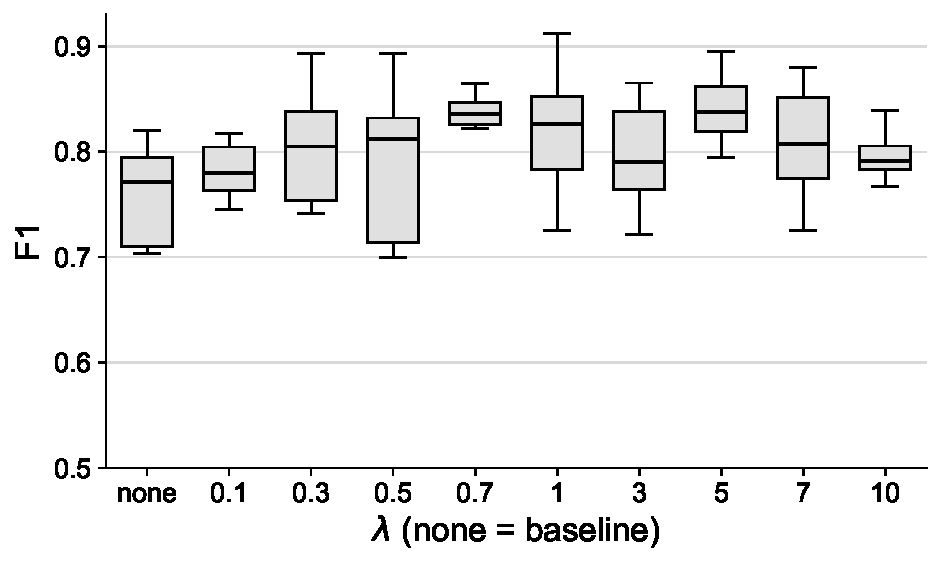
\includegraphics[width=1\linewidth]{boxplot_f1_none_vs_abs_lam.pdf}
\caption{Sensitivity of the detection F1 to the attention-constraint weight $\lambda$.}
\label{fig:lambda}
\end{figure}


\section{Generalization to an Additional Dataset}
\label{sec:generalization}

We retrain and evaluate our method on an additional public GPR dataset comprising 247 B-scan images,
following the same training and evaluation protocol described in Section~\ref{sec:impl}.
Table~\ref{tab:generalization} reports the resulting precision, recall, and F1-score.
The proposed method again outperforms the baseline, improving the F1-score from 0.75 to 0.79
and the precision from 0.68 to 0.76, while recall remains essentially unchanged.
This indicates that the benefit of explicit geometric attention supervision is not limited to the primary dataset
and consistently holds when the method is trained on a different GPR dataset.

\begin{table}[]
\caption{Detection performance on an additional GPR dataset.}
\label{tab:generalization}
\centering
\setlength{\tabcolsep}{4pt}
\begin{tabular}{lccc}
\toprule
Method & Precision & Recall & F1-score \\
\midrule
Baseline & $0.68 \pm 0.08$ & $0.83 \pm 0.04$ & $0.75 \pm 0.05$ \\
\textbf{Ours} & $\mathbf{0.76 \pm 0.06}$ & $0.83 \pm 0.06$ & $\mathbf{0.79 \pm 0.04}$ \\
\bottomrule
\end{tabular}
\end{table}

%\subsection{Result3}
%软性的约束是不是可能会更加好 如果lam参数调节好的话
\section{Discussion}
%讨论为什么不直接预测双曲线--面前主流的任务还是用bbox
%新课题中  首先是对于双曲线带的预测 用真实数据和模拟数据 双曲线带的重叠性 和  对应的矩阵的iou的。。。
%然后是对于双曲线参数的预测 真实数据预测 只和标注数据的参数 参数的话 厚度应该不需要
%模拟数据中加入正确的地下位置的模拟
\subsection{On the choice of output representation}
%我们的标注工具已经提供了每条双曲线完整的参数化描述,但是目前我们没有训练网络直接回归这些参数。

% 这是因为，第一,主流的检测任务及其数据集和评价协议(基于IoU的精确率、召回率与F1)都是围绕边界框构建的;
% 保留边界框输出使我们能够在完全一致的协议下与主流检测器和通用注意力模块进行公平比较。

% 第二,直接回归诸如曲率之类的双曲线参数对标注噪声、杂波、旁瓣以及相互重叠的回波都很敏感,
% 而且各参数尺度不一使得损失难以平衡。
Although our annotation tool provides a complete parametric description of each hyperbola,
in this work we do not train the network to regress these parameters directly, for two main reasons.
First, the mainstream detection task, together with its datasets and evaluation protocols (IoU-based
precision, recall, and F1), is built around bounding boxes; retaining a
bounding-box output therefore allows a fair comparison with mainstream detectors
and generic attention modules under a fully identical protocol. 
Second, directly regressing hyperbola parameters such as slope is sensitive to annotation
noise, clutter, side lobes, and mutually overlapping echoes, while the disparate
scales of the individual parameters make the training loss difficult to balance.


%这些替代方案构成了一个输出粒度的谱系。在一端,传统的基于对比度或边缘的提取方法配合霍夫变换或最小二乘拟合,能够显式地恢复曲线本身,但在杂波、旁瓣以及双曲线相互重叠的情况下十分脆弱,且依赖于细致的参数调节。边界框则位于另一端——粗糙,但鲁棒且高度标准化。像素级的分割掩膜介于两者之间:它能更紧地贴合回波轮廓,但需要密集的逐像素标注,难以在不同方法之间进行一致的比较,并且仍然无法给出双曲线的底层参数,如顶点位置或曲率。直接的参数化回归几何信息最丰富,却也最难稳定训练。因此,我们将网络的输出保持在边界框这一端,转而将更精细的条带几何作为监督信号注入网络,从而在保留标准检测器的鲁棒性与可比性的同时,仍能受益于几何先验;而真正恢复参数化的双曲线本身,则留待未来工作。


\subsection{Cross-dataset domain shift}
\label{sec:cross-dataset}
The generalization experiment in Section~\ref{sec:generalization} retrains the network from scratch on the additional dataset,
which confirms that the proposed attention supervision is beneficial regardless of which dataset it is trained on, 
but it does not probe how well a model trained on one dataset performs on the other \emph{without} retraining. 
To examine this more demanding setting, we train the network on one of the two datasets at a training ratio of 0.7 and,
without any fine-tuning, directly evaluate the resulting model on the other;
this is repeated in both directions, and all numbers below are averaged over ten random seeds.

Table~\ref{tab:cross-dataset} reports the results, reusing the in-domain F1 values already established
at this training ratio in Table~\ref{tab:bbox_results} (primary dataset) and Table~\ref{tab:generalization} (additional dataset).
Cross-dataset performance collapses sharply in both directions, with F1 falling to roughly 0.08--0.16.
The two datasets likely differ in more than the shape of the hyperbolas.
Acquisition equipment, subsurface conditions, and general B-scan appearance may all differ between them,
so neither model has learned anything that carries over to the other.


Such cross-dataset degradation is a well-documented difficulty in GPR interpretation more broadly,
and is not unique to hyperbola detection: it has motivated dedicated domain-adaptation techniques for GPR data inversion~\cite{rw-gpr-uda}
and for GPR object detection itself~\cite{rw-gpr-da},
as well as a range of transfer-learning strategies for related GPR recognition tasks~\cite{intro-tl-gpr1,intro-tl-gpr2,intro-tl-gpr3}.
Our approach does not adopt any of these dedicated domain-adaptation techniques;
the improvement observed above comes only from the explicit attention supervision described earlier.


\begin{table*}[]
\caption{Cross-dataset detection performance.}
\label{tab:cross-dataset}
\centering
\setlength{\tabcolsep}{4pt}
\begin{tabular}{llcccc}
\toprule
Train$\to$Test & Method & In-domain F1-score & Cross Precision & Cross Recall & Cross F1-score \\
\midrule
\multirow{2}{*}{Primary$\to$Additional} & Baseline & $0.68 \pm 0.20$ & $0.42 \pm 0.07$ & $0.05 \pm 0.02$ & $0.08 \pm 0.02$ \\
 & \textbf{Ours} & $0.84 \pm 0.03$ & $\mathbf{0.42 \pm 0.06}$ & $\mathbf{0.05 \pm 0.02}$ & $\mathbf{0.09 \pm 0.04}$ \\
\midrule
\multirow{2}{*}{Additional$\to$Primary} & Baseline & $0.75 \pm 0.05$ & $0.14 \pm 0.04$ & $0.14 \pm 0.04$ & $0.14 \pm 0.03$ \\
 & \textbf{Ours} & $0.79 \pm 0.04$ & $\mathbf{0.17 \pm 0.05}$ & $\mathbf{0.17 \pm 0.05}$ & $\mathbf{0.16 \pm 0.03}$ \\
\bottomrule
\end{tabular}
\end{table*}

\subsection{Future work}
%我们未来将对双曲线的参数进行预测，并输出各种参数用于反演
%反演的作用
%已经有一些输出参数的工作，比如。。。。
%对于我们的标注的双曲线带，一般的检测头可能不足够。。。
%我们将融合多种深度学习方法。。。
Although directly regressing hyperbola parameters is challenging for the reasons
discussed above, it remains the most informative output for practical use, and
overcoming this difficulty is a natural direction for future work: moving from
bounding-box localization toward predicting the parametric hyperbola itself and
exporting its parameters for inversion. In GPR interpretation, inversion aims to
recover the physical properties of a buried target from its hyperbolic signature: the apex position
and the opening of the curve are governed by the target depth and the
propagation velocity in the host medium, so that accurate parameters translate
into estimates of burial depth, object radius, and the dielectric permittivity of
the surrounding soil, which are the quantities of practical interest for utility
mapping and condition assessment~\cite{liu2022pipeline}.
Several recent studies already predict such hyperbola parameters directly instead of
boxes, for example through transformer-based regression~\cite{jin2024gprformer,ge2024gprtransunet}
or vertex-oriented keypoint and state-space formulations~\cite{hou2025endtoend,lan2024statespace}.
The quantities we would ultimately estimate, namely the apex position and the opening of the
curve, are essentially the same as those targeted by these works, so we do not claim a
new set of parameters to predict.
What differs is our starting point: we already have a complete parametric annotation of
each hyperbola band, so moving on to predict these parameters is a natural next step for us.
In addition, our attention branch is already supervised by the hyperbola-band mask to produce
a band-shaped response that closely follows the target geometry, which offers a natural bridge
toward such parametric prediction.
A promising direction is therefore to attach a lightweight regression head on top of this
response to decode the vertex, slope, span, and thickness of each hyperbola, rather than
building a separate parameter regressor from scratch, so that the model outputs the complete
parametric hyperbola end to end and directly supports downstream inversion.

%未来的工作是对双曲线进行预测,并输出各种参数用于反演:本文最直接的延伸是从边界框定位转向预测双曲线本身。由于注意力分支已经被监督为产生贴合双曲线几何的条带状响应,一个自然的下一步是在其上附加一个轻量的回归头,把该响应解码为每条双曲线的参数化描述——顶点位置、张开宽度、曲率与带状厚度,而不是轴对齐的矩形框。这样的参数化输出可以直接馈入下游的地球物理反演,从而无需单独的后处理曲线拟合阶段即可估计目标的埋深、半径以及埋藏介质属性。
% The most direct extension of this work is to move beyond bounding-box
% localization toward predicting the hyperbola itself. Because the attention
% branch is already supervised to produce a band-shaped response that closely
% follows the hyperbola geometry, a natural next step is to attach a lightweight
% regression head that decodes this response into the parametric description of
% each hyperbola---vertex position, opening width, curvature, and band
% thickness---rather than an axis-aligned box. Such parametric outputs would feed
% downstream geophysical inversion directly, enabling estimation of target depth,
% radius, and burial-medium properties without a separate post-hoc curve-fitting
% stage.

%第二个方向是考察本文的几何引导注意力监督在不同检测范式间的迁移能力:本文的检测器以稠密的YOLO风格回归框尺寸与中心偏移,而中心点式(如CenterNet风格)或基于关键点的检测器通过中心热力图来定位目标,其空间响应在本质上不同于条带状的注意力图。研究显式的条带监督如何与这类以中心为焦点的表示相互作用、以及是否仍然有益,将有助于厘清该方法的通用性,并指导其融入更广泛的探地雷达检测器。
% A second direction is to examine how the proposed geometry-guided attention
% supervision transfers across detection paradigms. Our current detector regresses
% box size and center offset in a dense YOLO-style manner, whereas center-point
% (e.g., CenterNet-style) or keypoint-based detectors localize targets through
% center heatmaps whose spatial response differs in nature from a band-shaped
% attention map. Investigating how explicit band supervision interacts with such
% center-focused representations, and whether it remains beneficial, would clarify
% the generality of the approach and guide its integration into a wider range of
% GPR detectors.


\section{Conclusion}
%结论:本文针对探地雷达B-scan中双曲线回波的检测问题,提出了两点贡献:一是面向双曲线带状目标的参数化可视化标注工具,它以少量可解释的控制描述双曲线,并可同时导出形状参数与边界框;二是双曲线注意力网络,通过由双曲线条带掩膜显式监督的注意力分支,将几何先验注入特征表示,同时保留标准的边界框检测头。在公开GPR数据集上,所提方法在各训练数据比例下均优于基线:在0.7比例下F1由0.68提升至0.84,标准差由0.21降至0.03,增益主要来自召回率的提升;并取得0.89的最高F1,优于SE、CBAM、Non-local与坐标注意力等通用注意力模块。参数敏感性分析表明方法在较宽的约束权重区间内稳定有效。总体而言,以几何作为监督、而非直接改变输出表示,是一种简单而有效地利用双曲线结构先验的方式,并能保持与主流检测器的可比性。
%这是加入了两点改进(强化稳定性论述的意义、平滑future work的过渡)的修改版:

In this paper, we proposed a hyperbola-band attention method to improve hyperbola detection in GPR B-scan images. 
We first developed a dedicated annotation tool that describes each hyperbola 
as a parametric band through a few interpretable controls and exports both the shape parameters and the derived bounding box. Building on a standard bounding-box detector, we introduced an attention branch explicitly supervised by the hyperbola-band mask, injecting the geometric prior into the feature representation and thereby improving detection performance.
Experiments on a public GPR dataset show that the proposed supervision consistently improves detection across training-data ratios. At a training-data ratio of 0.7, it raises the F1-score from 0.68 to 0.84, with the gain driven mainly by higher recall. The standard deviation across random seeds is also reduced from 0.21 to 0.03, indicating that the geometric supervision stabilizes training and reduces sensitivity to initialization, which is particularly valuable under limited training data. The method also outperforms other attention mechanisms, confirming its effectiveness. While the current work focuses on localizing and classifying hyperbolas, future work will extend the framework to infer the hyperbola's shape parameters directly, meeting the requirements of downstream tasks such as geophysical inversion.

%In this paper, we proposed a hyperbola-band attention method to improve hyperbola detection in GPR B-scan images. We first developed a dedicated annotation tool that describes each hyperbola as a parametric band through a few interpretable controls and exports both the shape parameters and the derived bounding box. Building on a standard bounding-box detector, we then introduced an attention branch that is explicitly supervised by the hyperbola-band mask, injecting the geometric prior into the feature representation and thereby improving detection performance.

%Experiments on a public GPR dataset show that the proposed supervision consistently improves detection across training-data ratios. At a training-data ratio of 0.7, it raises the F1-score from 0.68 to 0.84 and reduces its standard deviation across random seeds from 0.21 to 0.03, with the gain driven mainly by higher recall. The method also outperforms other attention mechanisms, confirming its effectiveness. In future work, we will infer the parameters of the hyperbola itself to meet the requirements of downstream tasks such as geophysical inversion.



\section*{Acknowledgments}
This research was funded under the Japanese Research Fund Kakenhi-C 23K04329: Electromagnetic Detection and Velocimetry of Wood debris Moving in Water for Drifted Wood Disaster Reduction.


%{\appendices
%\section*{Proof of the First Zonklar Equation}
%Appendix one text goes here.
% You can choose not to have a title for an appendix if you want by leaving the argument blank
%\section*{Proof of the Second Zonklar Equation}
%Appendix two text goes here.}



\bibliographystyle{IEEEtran}
\bibliography{1references}


% \newpage

% \section{Biography Section}
% If you have an EPS/PDF photo (graphicx package needed), extra braces are
%  needed around the contents of the optional argument to biography to prevent
%  the LaTeX parser from getting confused when it sees the complicated
%  $\backslash${\tt{includegraphics}} command within an optional argument. (You can create
%  your own custom macro containing the $\backslash${\tt{includegraphics}} command to make things
%  simpler here.)
 
% \vspace{11pt}

% \bf{If you include a photo:}\vspace{-33pt}
% \begin{IEEEbiography}[{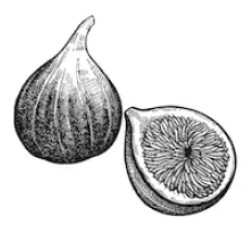
\includegraphics[width=1in,height=1.25in,clip,keepaspectratio]{fig1}}]{Michael Shell}
% Use $\backslash${\tt{begin\{IEEEbiography\}}} and then for the 1st argument use $\backslash${\tt{includegraphics}} to declare and link the author photo.
% Use the author name as the 3rd argument followed by the biography text.
% \end{IEEEbiography}

% \vspace{11pt}

% \bf{If you will not include a photo:}\vspace{-33pt}
% \begin{IEEEbiographynophoto}{John Doe}
% Use $\backslash${\tt{begin\{IEEEbiographynophoto\}}} and the author name as the argument followed by the biography text.
% \end{IEEEbiographynophoto}




\vfill

\end{document}


